%% PFG submission (Springer Nature LaTeX template, sn-basic author-year). Generated by build_pfg.py from ../main.tex.
\documentclass[pdflatex,sn-basic]{sn-jnl}

\usepackage{graphicx}
\usepackage{amsmath,amssymb}
\usepackage{booktabs}
\usepackage{xcolor}
\usepackage[T1]{fontenc}
\usepackage{lmodern}
\usepackage{enumitem}
\usepackage{float}
\usepackage[section]{placeins}
\input{glyphtounicode}
\pdfgentounicode=1
\graphicspath{{../}}
\raggedbottom
\renewcommand{\topfraction}{0.95}\renewcommand{\bottomfraction}{0.9}\renewcommand{\textfraction}{0.05}\renewcommand{\floatpagefraction}{0.85}

% Generated by make_paper_numbers.py from measured results. Do not edit by hand.
\newcommand{\BestEpMax}{4}
\newcommand{\BestEpMed}{1}
\newcommand{\BestEpMin}{1}
\newcommand{\BestEpN}{9}
\newcommand{\BestEpOne}{7}
\newcommand{\BestMAPA}{Source-only}
\newcommand{\BestMARO}{Source-only}
\newcommand{\BestPAMA}{+\, BN-TTA}
\newcommand{\BestPARO}{FDA scale 1.0 +\, BN-TTA}
\newcommand{\BestROMA}{FDA mix50}
\newcommand{\BestROPA}{FDA scale 1.0}
\newcommand{\DefMA}{4.93}
\newcommand{\DefPA}{4.30}
\newcommand{\DefRO}{5.66}
\newcommand{\FDABinsFiveTwelve}{100}
\newcommand{\FDASwapPct}{0.038}
\newcommand{\FDATilesMA}{12}
\newcommand{\FDATilesPA}{18}
\newcommand{\FDATilesRO}{55}
\newcommand{\FDATotalFiveTwelve}{262{,}144}
\newcommand{\FDAUnstyledMA}{0}
\newcommand{\FDAUnstyledPA}{8}
\newcommand{\FDAUnstyledPctMA}{0.0}
\newcommand{\FDAUnstyledPctPA}{8.3}
\newcommand{\FDAUnstyledPctRO}{0.2}
\newcommand{\FDAUnstyledRO}{5}
\newcommand{\HMA}{1719}
\newcommand{\HPA}{1100}
\newcommand{\HRO}{2554}
\newcommand{\InDomMAM}{0.582}
\newcommand{\InDomMAS}{0.069}
\newcommand{\InDomPAM}{0.747}
\newcommand{\InDomPAS}{0.012}
\newcommand{\InDomROM}{0.608}
\newcommand{\InDomROS}{0.009}
\newcommand{\MIXAPAllD}{$-$0.011}
\newcommand{\MIXAPAllN}{18}
\newcommand{\MIXAPAllW}{7}
\newcommand{\MIXAPMAPAD}{$-$0.010}
\newcommand{\MIXAPMAPAM}{0.791}
\newcommand{\MIXAPMAPAN}{3}
\newcommand{\MIXAPMAPAS}{0.001}
\newcommand{\MIXAPMAPAW}{1}
\newcommand{\MIXAPMAROD}{$-$0.233}
\newcommand{\MIXAPMAROM}{0.160}
\newcommand{\MIXAPMARON}{3}
\newcommand{\MIXAPMAROS}{0.022}
\newcommand{\MIXAPMAROW}{0}
\newcommand{\MIXAPPAMAD}{$-$0.147}
\newcommand{\MIXAPPAMAM}{0.595}
\newcommand{\MIXAPPAMAN}{3}
\newcommand{\MIXAPPAMAS}{0.044}
\newcommand{\MIXAPPAMAW}{0}
\newcommand{\MIXAPPAROD}{+0.008}
\newcommand{\MIXAPPAROM}{0.116}
\newcommand{\MIXAPPARON}{3}
\newcommand{\MIXAPPAROS}{0.028}
\newcommand{\MIXAPPAROW}{1}
\newcommand{\MIXAPROMAD}{$-$0.025}
\newcommand{\MIXAPROMAM}{0.370}
\newcommand{\MIXAPROMAN}{3}
\newcommand{\MIXAPROMAS}{0.054}
\newcommand{\MIXAPROMAW}{2}
\newcommand{\MIXAPROPAD}{+0.340}
\newcommand{\MIXAPROPAM}{0.626}
\newcommand{\MIXAPROPAN}{3}
\newcommand{\MIXAPROPAS}{0.048}
\newcommand{\MIXAPROPAW}{3}
\newcommand{\MIXAPSrcMAD}{$-$0.121}
\newcommand{\MIXAPSrcMAL}{5}
\newcommand{\MIXAPSrcMAN}{6}
\newcommand{\MIXAPSrcMAW}{1}
\newcommand{\MIXAPSrcPAD}{$-$0.069}
\newcommand{\MIXAPSrcPAL}{5}
\newcommand{\MIXAPSrcPAN}{6}
\newcommand{\MIXAPSrcPAW}{1}
\newcommand{\MIXAPSrcROD}{+0.157}
\newcommand{\MIXAPSrcROL}{1}
\newcommand{\MIXAPSrcRON}{6}
\newcommand{\MIXAPSrcROW}{5}
\newcommand{\MIXAllD}{+0.043}
\newcommand{\MIXAllN}{18}
\newcommand{\MIXAllW}{8}
\newcommand{\MIXMAPAD}{$-$0.012}
\newcommand{\MIXMAPAM}{0.699}
\newcommand{\MIXMAPAN}{3}
\newcommand{\MIXMAPAS}{0.005}
\newcommand{\MIXMAPAW}{1}
\newcommand{\MIXMAROD}{$-$0.199}
\newcommand{\MIXMAROM}{0.208}
\newcommand{\MIXMARON}{3}
\newcommand{\MIXMAROS}{0.044}
\newcommand{\MIXMAROW}{0}
\newcommand{\MIXPAMAD}{+0.025}
\newcommand{\MIXPAMAM}{0.343}
\newcommand{\MIXPAMAN}{3}
\newcommand{\MIXPAMAS}{0.101}
\newcommand{\MIXPAMAW}{1}
\newcommand{\MIXPAROD}{+0.014}
\newcommand{\MIXPAROM}{0.145}
\newcommand{\MIXPARON}{3}
\newcommand{\MIXPAROS}{0.025}
\newcommand{\MIXPAROW}{1}
\newcommand{\MIXPAllD}{+0.043}
\newcommand{\MIXPAllN}{18}
\newcommand{\MIXPAllW}{9}
\newcommand{\MIXPMAPAD}{$-$0.003}
\newcommand{\MIXPMAPAM}{0.675}
\newcommand{\MIXPMAPAN}{3}
\newcommand{\MIXPMAPAS}{0.057}
\newcommand{\MIXPMAPAW}{1}
\newcommand{\MIXPMAROD}{$-$0.180}
\newcommand{\MIXPMAROM}{0.177}
\newcommand{\MIXPMARON}{3}
\newcommand{\MIXPMAROS}{0.042}
\newcommand{\MIXPMAROW}{0}
\newcommand{\MIXPPAMAD}{+0.022}
\newcommand{\MIXPPAMAM}{0.220}
\newcommand{\MIXPPAMAN}{3}
\newcommand{\MIXPPAMAS}{0.082}
\newcommand{\MIXPPAMAW}{1}
\newcommand{\MIXPPAROD}{+0.026}
\newcommand{\MIXPPAROM}{0.122}
\newcommand{\MIXPPARON}{3}
\newcommand{\MIXPPAROS}{0.024}
\newcommand{\MIXPPAROW}{2}
\newcommand{\MIXPROMAD}{+0.114}
\newcommand{\MIXPROMAM}{0.258}
\newcommand{\MIXPROMAN}{3}
\newcommand{\MIXPROMAS}{0.043}
\newcommand{\MIXPROMAW}{2}
\newcommand{\MIXPROPAD}{+0.278}
\newcommand{\MIXPROPAM}{0.480}
\newcommand{\MIXPROPAN}{3}
\newcommand{\MIXPROPAS}{0.067}
\newcommand{\MIXPROPAW}{3}
\newcommand{\MIXRAllD}{$-$0.004}
\newcommand{\MIXRAllN}{18}
\newcommand{\MIXRAllW}{8}
\newcommand{\MIXRMAPAD}{$-$0.021}
\newcommand{\MIXRMAPAM}{0.731}
\newcommand{\MIXRMAPAN}{3}
\newcommand{\MIXRMAPAS}{0.069}
\newcommand{\MIXRMAPAW}{2}
\newcommand{\MIXRMAROD}{$-$0.210}
\newcommand{\MIXRMAROM}{0.265}
\newcommand{\MIXRMARON}{3}
\newcommand{\MIXRMAROS}{0.082}
\newcommand{\MIXRMAROW}{0}
\newcommand{\MIXROMAD}{+0.141}
\newcommand{\MIXROMAM}{0.376}
\newcommand{\MIXROMAN}{3}
\newcommand{\MIXROMAS}{0.043}
\newcommand{\MIXROMAW}{2}
\newcommand{\MIXROPAD}{+0.288}
\newcommand{\MIXROPAM}{0.537}
\newcommand{\MIXROPAN}{3}
\newcommand{\MIXROPAS}{0.014}
\newcommand{\MIXROPAW}{3}
\newcommand{\MIXRPAMAD}{$-$0.028}
\newcommand{\MIXRPAMAM}{0.852}
\newcommand{\MIXRPAMAN}{3}
\newcommand{\MIXRPAMAS}{0.065}
\newcommand{\MIXRPAMAW}{1}
\newcommand{\MIXRPAROD}{$-$0.018}
\newcommand{\MIXRPAROM}{0.195}
\newcommand{\MIXRPARON}{3}
\newcommand{\MIXRPAROS}{0.072}
\newcommand{\MIXRPAROW}{1}
\newcommand{\MIXRROMAD}{$-$0.001}
\newcommand{\MIXRROMAM}{0.704}
\newcommand{\MIXRROMAN}{3}
\newcommand{\MIXRROMAS}{0.037}
\newcommand{\MIXRROMAW}{1}
\newcommand{\MIXRROPAD}{+0.254}
\newcommand{\MIXRROPAM}{0.628}
\newcommand{\MIXRROPAN}{3}
\newcommand{\MIXRROPAS}{0.087}
\newcommand{\MIXRROPAW}{3}
\newcommand{\MIXSrcMAD}{$-$0.106}
\newcommand{\MIXSrcMAL}{5}
\newcommand{\MIXSrcMAN}{6}
\newcommand{\MIXSrcMAW}{1}
\newcommand{\MIXSrcPAD}{+0.020}
\newcommand{\MIXSrcPAL}{4}
\newcommand{\MIXSrcPAN}{6}
\newcommand{\MIXSrcPAW}{2}
\newcommand{\MIXSrcROD}{+0.214}
\newcommand{\MIXSrcROL}{1}
\newcommand{\MIXSrcRON}{6}
\newcommand{\MIXSrcROW}{5}
\newcommand{\MIXTTAAPAllD}{+0.013}
\newcommand{\MIXTTAAPAllN}{18}
\newcommand{\MIXTTAAPAllW}{9}
\newcommand{\MIXTTAAPMAPAD}{$-$0.023}
\newcommand{\MIXTTAAPMAPAM}{0.778}
\newcommand{\MIXTTAAPMAPAN}{3}
\newcommand{\MIXTTAAPMAPAS}{0.025}
\newcommand{\MIXTTAAPMAPAW}{1}
\newcommand{\MIXTTAAPMAROD}{$-$0.161}
\newcommand{\MIXTTAAPMAROM}{0.232}
\newcommand{\MIXTTAAPMARON}{3}
\newcommand{\MIXTTAAPMAROS}{0.008}
\newcommand{\MIXTTAAPMAROW}{0}
\newcommand{\MIXTTAAPPAMAD}{$-$0.145}
\newcommand{\MIXTTAAPPAMAM}{0.597}
\newcommand{\MIXTTAAPPAMAN}{3}
\newcommand{\MIXTTAAPPAMAS}{0.048}
\newcommand{\MIXTTAAPPAMAW}{0}
\newcommand{\MIXTTAAPPAROD}{+0.047}
\newcommand{\MIXTTAAPPAROM}{0.154}
\newcommand{\MIXTTAAPPARON}{3}
\newcommand{\MIXTTAAPPAROS}{0.040}
\newcommand{\MIXTTAAPPAROW}{3}
\newcommand{\MIXTTAAPROMAD}{+0.009}
\newcommand{\MIXTTAAPROMAM}{0.404}
\newcommand{\MIXTTAAPROMAN}{3}
\newcommand{\MIXTTAAPROMAS}{0.102}
\newcommand{\MIXTTAAPROMAW}{2}
\newcommand{\MIXTTAAPROPAD}{+0.350}
\newcommand{\MIXTTAAPROPAM}{0.636}
\newcommand{\MIXTTAAPROPAN}{3}
\newcommand{\MIXTTAAPROPAS}{0.031}
\newcommand{\MIXTTAAPROPAW}{3}
\newcommand{\MIXTTAAllD}{$-$0.010}
\newcommand{\MIXTTAAllN}{18}
\newcommand{\MIXTTAAllW}{9}
\newcommand{\MIXTTAMAPAD}{$-$0.150}
\newcommand{\MIXTTAMAPAM}{0.561}
\newcommand{\MIXTTAMAPAN}{3}
\newcommand{\MIXTTAMAPAS}{0.047}
\newcommand{\MIXTTAMAPAW}{0}
\newcommand{\MIXTTAMAROD}{$-$0.149}
\newcommand{\MIXTTAMAROM}{0.257}
\newcommand{\MIXTTAMARON}{3}
\newcommand{\MIXTTAMAROS}{0.013}
\newcommand{\MIXTTAMAROW}{0}
\newcommand{\MIXTTAPAMAD}{+0.042}
\newcommand{\MIXTTAPAMAM}{0.359}
\newcommand{\MIXTTAPAMAN}{3}
\newcommand{\MIXTTAPAMAS}{0.084}
\newcommand{\MIXTTAPAMAW}{2}
\newcommand{\MIXTTAPAROD}{+0.050}
\newcommand{\MIXTTAPAROM}{0.181}
\newcommand{\MIXTTAPARON}{3}
\newcommand{\MIXTTAPAROS}{0.029}
\newcommand{\MIXTTAPAROW}{3}
\newcommand{\MIXTTAPAllD}{$-$0.058}
\newcommand{\MIXTTAPAllN}{18}
\newcommand{\MIXTTAPAllW}{9}
\newcommand{\MIXTTAPMAPAD}{$-$0.277}
\newcommand{\MIXTTAPMAPAM}{0.401}
\newcommand{\MIXTTAPMAPAN}{3}
\newcommand{\MIXTTAPMAPAS}{0.050}
\newcommand{\MIXTTAPMAPAW}{0}
\newcommand{\MIXTTAPMAROD}{$-$0.189}
\newcommand{\MIXTTAPMAROM}{0.168}
\newcommand{\MIXTTAPMARON}{3}
\newcommand{\MIXTTAPMAROS}{0.013}
\newcommand{\MIXTTAPMAROW}{0}
\newcommand{\MIXTTAPPAMAD}{+0.037}
\newcommand{\MIXTTAPPAMAM}{0.235}
\newcommand{\MIXTTAPPAMAN}{3}
\newcommand{\MIXTTAPPAMAS}{0.073}
\newcommand{\MIXTTAPPAMAW}{2}
\newcommand{\MIXTTAPPAROD}{+0.037}
\newcommand{\MIXTTAPPAROM}{0.133}
\newcommand{\MIXTTAPPARON}{3}
\newcommand{\MIXTTAPPAROS}{0.018}
\newcommand{\MIXTTAPPAROW}{3}
\newcommand{\MIXTTAPROMAD}{+0.018}
\newcommand{\MIXTTAPROMAM}{0.162}
\newcommand{\MIXTTAPROMAN}{3}
\newcommand{\MIXTTAPROMAS}{0.017}
\newcommand{\MIXTTAPROMAW}{2}
\newcommand{\MIXTTAPROPAD}{+0.029}
\newcommand{\MIXTTAPROPAM}{0.231}
\newcommand{\MIXTTAPROPAN}{3}
\newcommand{\MIXTTAPROPAS}{0.023}
\newcommand{\MIXTTAPROPAW}{2}
\newcommand{\MIXTTARAllD}{+0.139}
\newcommand{\MIXTTARAllN}{18}
\newcommand{\MIXTTARAllW}{14}
\newcommand{\MIXTTARMAPAD}{+0.187}
\newcommand{\MIXTTARMAPAM}{0.939}
\newcommand{\MIXTTARMAPAN}{3}
\newcommand{\MIXTTARMAPAS}{0.025}
\newcommand{\MIXTTARMAPAW}{3}
\newcommand{\MIXTTARMAROD}{+0.076}
\newcommand{\MIXTTARMAROM}{0.552}
\newcommand{\MIXTTARMARON}{3}
\newcommand{\MIXTTARMAROS}{0.060}
\newcommand{\MIXTTARMAROW}{3}
\newcommand{\MIXTTAROMAD}{+0.035}
\newcommand{\MIXTTAROMAM}{0.270}
\newcommand{\MIXTTAROMAN}{3}
\newcommand{\MIXTTAROMAS}{0.025}
\newcommand{\MIXTTAROMAW}{2}
\newcommand{\MIXTTAROPAD}{+0.111}
\newcommand{\MIXTTAROPAM}{0.360}
\newcommand{\MIXTTAROPAN}{3}
\newcommand{\MIXTTAROPAS}{0.029}
\newcommand{\MIXTTAROPAW}{2}
\newcommand{\MIXTTARPAMAD}{$-$0.072}
\newcommand{\MIXTTARPAMAM}{0.807}
\newcommand{\MIXTTARPAMAN}{3}
\newcommand{\MIXTTARPAMAS}{0.044}
\newcommand{\MIXTTARPAMAW}{0}
\newcommand{\MIXTTARPAROD}{+0.071}
\newcommand{\MIXTTARPAROM}{0.284}
\newcommand{\MIXTTARPARON}{3}
\newcommand{\MIXTTARPAROS}{0.066}
\newcommand{\MIXTTARPAROW}{2}
\newcommand{\MIXTTARROMAD}{+0.119}
\newcommand{\MIXTTARROMAM}{0.825}
\newcommand{\MIXTTARROMAN}{3}
\newcommand{\MIXTTARROMAS}{0.026}
\newcommand{\MIXTTARROMAW}{3}
\newcommand{\MIXTTARROPAD}{+0.453}
\newcommand{\MIXTTARROPAM}{0.827}
\newcommand{\MIXTTARROPAN}{3}
\newcommand{\MIXTTARROPAS}{0.061}
\newcommand{\MIXTTARROPAW}{3}
\newcommand{\MIXTTAvsMIXAPD}{+0.024}
\newcommand{\MIXTTAvsMIXAPN}{18}
\newcommand{\MIXTTAvsMIXAPW}{13}
\newcommand{\MIXTTAvsMIXD}{$-$0.053}
\newcommand{\MIXTTAvsMIXN}{18}
\newcommand{\MIXTTAvsMIXW}{7}
\newcommand{\NoDataMA}{0.000}
\newcommand{\NoDataPA}{0.000}
\newcommand{\NoDataRO}{0.039}
\newcommand{\ONEAPAllD}{$-$0.020}
\newcommand{\ONEAPAllN}{18}
\newcommand{\ONEAPAllW}{8}
\newcommand{\ONEAPMAPAD}{$-$0.027}
\newcommand{\ONEAPMAPAM}{0.773}
\newcommand{\ONEAPMAPAN}{3}
\newcommand{\ONEAPMAPAS}{0.019}
\newcommand{\ONEAPMAPAW}{0}
\newcommand{\ONEAPMAROD}{$-$0.224}
\newcommand{\ONEAPMAROM}{0.169}
\newcommand{\ONEAPMARON}{3}
\newcommand{\ONEAPMAROS}{0.018}
\newcommand{\ONEAPMAROW}{0}
\newcommand{\ONEAPPAMAD}{$-$0.215}
\newcommand{\ONEAPPAMAM}{0.527}
\newcommand{\ONEAPPAMAN}{3}
\newcommand{\ONEAPPAMAS}{0.039}
\newcommand{\ONEAPPAMAW}{0}
\newcommand{\ONEAPPAROD}{+0.034}
\newcommand{\ONEAPPAROM}{0.141}
\newcommand{\ONEAPPARON}{3}
\newcommand{\ONEAPPAROS}{0.020}
\newcommand{\ONEAPPAROW}{3}
\newcommand{\ONEAPROMAD}{$-$0.018}
\newcommand{\ONEAPROMAM}{0.378}
\newcommand{\ONEAPROMAN}{3}
\newcommand{\ONEAPROMAS}{0.044}
\newcommand{\ONEAPROMAW}{2}
\newcommand{\ONEAPROPAD}{+0.328}
\newcommand{\ONEAPROPAM}{0.614}
\newcommand{\ONEAPROPAN}{3}
\newcommand{\ONEAPROPAS}{0.021}
\newcommand{\ONEAPROPAW}{3}
\newcommand{\ONEAPSrcMAD}{$-$0.126}
\newcommand{\ONEAPSrcMAL}{6}
\newcommand{\ONEAPSrcMAN}{6}
\newcommand{\ONEAPSrcMAW}{0}
\newcommand{\ONEAPSrcPAD}{$-$0.091}
\newcommand{\ONEAPSrcPAL}{3}
\newcommand{\ONEAPSrcPAN}{6}
\newcommand{\ONEAPSrcPAW}{3}
\newcommand{\ONEAPSrcROD}{+0.155}
\newcommand{\ONEAPSrcROL}{1}
\newcommand{\ONEAPSrcRON}{6}
\newcommand{\ONEAPSrcROW}{5}
\newcommand{\ONEAllD}{+0.037}
\newcommand{\ONEAllN}{18}
\newcommand{\ONEAllW}{11}
\newcommand{\ONEMAPAD}{$-$0.025}
\newcommand{\ONEMAPAM}{0.686}
\newcommand{\ONEMAPAN}{3}
\newcommand{\ONEMAPAS}{0.020}
\newcommand{\ONEMAPAW}{1}
\newcommand{\ONEMAROD}{$-$0.167}
\newcommand{\ONEMAROM}{0.239}
\newcommand{\ONEMARON}{3}
\newcommand{\ONEMAROS}{0.012}
\newcommand{\ONEMAROW}{0}
\newcommand{\ONEPAMAAPHi}{0.567}
\newcommand{\ONEPAMAAPLo}{0.489}
\newcommand{\ONEPAMAD}{$-$0.043}
\newcommand{\ONEPAMAFRange}{0.0005}
\newcommand{\ONEPAMAM}{0.274}
\newcommand{\ONEPAMAN}{3}
\newcommand{\ONEPAMAS}{0.000}
\newcommand{\ONEPAMAW}{2}
\newcommand{\ONEPAROD}{+0.060}
\newcommand{\ONEPAROM}{0.191}
\newcommand{\ONEPARON}{3}
\newcommand{\ONEPAROS}{0.032}
\newcommand{\ONEPAROW}{3}
\newcommand{\ONEPAllD}{+0.058}
\newcommand{\ONEPAllN}{18}
\newcommand{\ONEPAllW}{14}
\newcommand{\ONEPMAPAD}{+0.042}
\newcommand{\ONEPMAPAM}{0.720}
\newcommand{\ONEPMAPAN}{3}
\newcommand{\ONEPMAPAS}{0.043}
\newcommand{\ONEPMAPAW}{3}
\newcommand{\ONEPMAROD}{$-$0.124}
\newcommand{\ONEPMAROM}{0.233}
\newcommand{\ONEPMARON}{3}
\newcommand{\ONEPMAROS}{0.054}
\newcommand{\ONEPMAROW}{1}
\newcommand{\ONEPPAMAD}{$-$0.035}
\newcommand{\ONEPPAMAM}{0.163}
\newcommand{\ONEPPAMAN}{3}
\newcommand{\ONEPPAMAS}{0.001}
\newcommand{\ONEPPAMAW}{2}
\newcommand{\ONEPPAROD}{+0.054}
\newcommand{\ONEPPAROM}{0.150}
\newcommand{\ONEPPARON}{3}
\newcommand{\ONEPPAROS}{0.043}
\newcommand{\ONEPPAROW}{3}
\newcommand{\ONEPROMAD}{+0.065}
\newcommand{\ONEPROMAM}{0.209}
\newcommand{\ONEPROMAN}{3}
\newcommand{\ONEPROMAS}{0.042}
\newcommand{\ONEPROMAW}{2}
\newcommand{\ONEPROPAD}{+0.347}
\newcommand{\ONEPROPAM}{0.549}
\newcommand{\ONEPROPAN}{3}
\newcommand{\ONEPROPAS}{0.095}
\newcommand{\ONEPROPAW}{3}
\newcommand{\ONERAllD}{+0.002}
\newcommand{\ONERAllN}{18}
\newcommand{\ONERAllW}{9}
\newcommand{\ONERMAPAD}{$-$0.095}
\newcommand{\ONERMAPAM}{0.657}
\newcommand{\ONERMAPAN}{3}
\newcommand{\ONERMAPAS}{0.036}
\newcommand{\ONERMAPAW}{0}
\newcommand{\ONERMAROD}{$-$0.206}
\newcommand{\ONERMAROM}{0.270}
\newcommand{\ONERMARON}{3}
\newcommand{\ONERMAROS}{0.086}
\newcommand{\ONERMAROW}{0}
\newcommand{\ONEROMAD}{+0.093}
\newcommand{\ONEROMAM}{0.328}
\newcommand{\ONEROMAN}{3}
\newcommand{\ONEROMAS}{0.051}
\newcommand{\ONEROMAW}{2}
\newcommand{\ONEROPAD}{+0.302}
\newcommand{\ONEROPAM}{0.551}
\newcommand{\ONEROPAN}{3}
\newcommand{\ONEROPAS}{0.021}
\newcommand{\ONEROPAW}{3}
\newcommand{\ONERPAMAD}{$-$0.024}
\newcommand{\ONERPAMAM}{0.855}
\newcommand{\ONERPAMAN}{3}
\newcommand{\ONERPAMAS}{0.016}
\newcommand{\ONERPAMAW}{1}
\newcommand{\ONERPAROD}{+0.071}
\newcommand{\ONERPAROM}{0.284}
\newcommand{\ONERPARON}{3}
\newcommand{\ONERPAROS}{0.039}
\newcommand{\ONERPAROW}{2}
\newcommand{\ONERROMAD}{+0.071}
\newcommand{\ONERROMAM}{0.776}
\newcommand{\ONERROMAN}{3}
\newcommand{\ONERROMAS}{0.012}
\newcommand{\ONERROMAW}{3}
\newcommand{\ONERROPAD}{+0.196}
\newcommand{\ONERROPAM}{0.570}
\newcommand{\ONERROPAN}{3}
\newcommand{\ONERROPAS}{0.082}
\newcommand{\ONERROPAW}{3}
\newcommand{\ONESrcMAD}{$-$0.096}
\newcommand{\ONESrcMAL}{5}
\newcommand{\ONESrcMAN}{6}
\newcommand{\ONESrcMAW}{1}
\newcommand{\ONESrcPAD}{+0.008}
\newcommand{\ONESrcPAL}{1}
\newcommand{\ONESrcPAN}{6}
\newcommand{\ONESrcPAW}{5}
\newcommand{\ONESrcROD}{+0.197}
\newcommand{\ONESrcROL}{1}
\newcommand{\ONESrcRON}{6}
\newcommand{\ONESrcROW}{5}
\newcommand{\ONETTAAPAllD}{$-$0.026}
\newcommand{\ONETTAAPAllN}{18}
\newcommand{\ONETTAAPAllW}{7}
\newcommand{\ONETTAAPMAPAD}{$-$0.072}
\newcommand{\ONETTAAPMAPAM}{0.729}
\newcommand{\ONETTAAPMAPAN}{3}
\newcommand{\ONETTAAPMAPAS}{0.037}
\newcommand{\ONETTAAPMAPAW}{0}
\newcommand{\ONETTAAPMAROD}{$-$0.153}
\newcommand{\ONETTAAPMAROM}{0.241}
\newcommand{\ONETTAAPMARON}{3}
\newcommand{\ONETTAAPMAROS}{0.041}
\newcommand{\ONETTAAPMAROW}{0}
\newcommand{\ONETTAAPPAMAD}{$-$0.239}
\newcommand{\ONETTAAPPAMAM}{0.503}
\newcommand{\ONETTAAPPAMAN}{3}
\newcommand{\ONETTAAPPAMAS}{0.043}
\newcommand{\ONETTAAPPAMAW}{0}
\newcommand{\ONETTAAPPAROD}{+0.056}
\newcommand{\ONETTAAPPAROM}{0.163}
\newcommand{\ONETTAAPPARON}{3}
\newcommand{\ONETTAAPPAROS}{0.019}
\newcommand{\ONETTAAPPAROW}{3}
\newcommand{\ONETTAAPROMAD}{$-$0.047}
\newcommand{\ONETTAAPROMAM}{0.348}
\newcommand{\ONETTAAPROMAN}{3}
\newcommand{\ONETTAAPROMAS}{0.039}
\newcommand{\ONETTAAPROMAW}{1}
\newcommand{\ONETTAAPROPAD}{+0.300}
\newcommand{\ONETTAAPROPAM}{0.586}
\newcommand{\ONETTAAPROPAN}{3}
\newcommand{\ONETTAAPROPAS}{0.027}
\newcommand{\ONETTAAPROPAW}{3}
\newcommand{\ONETTAAllD}{$-$0.042}
\newcommand{\ONETTAAllN}{18}
\newcommand{\ONETTAAllW}{9}
\newcommand{\ONETTAMAPAD}{$-$0.241}
\newcommand{\ONETTAMAPAM}{0.470}
\newcommand{\ONETTAMAPAN}{3}
\newcommand{\ONETTAMAPAS}{0.058}
\newcommand{\ONETTAMAPAW}{0}
\newcommand{\ONETTAMAROD}{$-$0.127}
\newcommand{\ONETTAMAROM}{0.280}
\newcommand{\ONETTAMARON}{3}
\newcommand{\ONETTAMAROS}{0.022}
\newcommand{\ONETTAMAROW}{0}
\newcommand{\ONETTAPAMAD}{$-$0.043}
\newcommand{\ONETTAPAMAM}{0.274}
\newcommand{\ONETTAPAMAN}{3}
\newcommand{\ONETTAPAMAS}{0.031}
\newcommand{\ONETTAPAMAW}{2}
\newcommand{\ONETTAPAROD}{+0.070}
\newcommand{\ONETTAPAROM}{0.201}
\newcommand{\ONETTAPARON}{3}
\newcommand{\ONETTAPAROS}{0.033}
\newcommand{\ONETTAPAROW}{3}
\newcommand{\ONETTAPAllD}{$-$0.084}
\newcommand{\ONETTAPAllN}{18}
\newcommand{\ONETTAPAllW}{9}
\newcommand{\ONETTAPMAPAD}{$-$0.361}
\newcommand{\ONETTAPMAPAM}{0.317}
\newcommand{\ONETTAPMAPAN}{3}
\newcommand{\ONETTAPMAPAS}{0.050}
\newcommand{\ONETTAPMAPAW}{0}
\newcommand{\ONETTAPMAROD}{$-$0.172}
\newcommand{\ONETTAPMAROM}{0.185}
\newcommand{\ONETTAPMARON}{3}
\newcommand{\ONETTAPMAROS}{0.013}
\newcommand{\ONETTAPMAROW}{0}
\newcommand{\ONETTAPPAMAD}{$-$0.033}
\newcommand{\ONETTAPPAMAM}{0.165}
\newcommand{\ONETTAPPAMAN}{3}
\newcommand{\ONETTAPPAMAS}{0.023}
\newcommand{\ONETTAPPAMAW}{2}
\newcommand{\ONETTAPPAROD}{+0.051}
\newcommand{\ONETTAPPAROM}{0.148}
\newcommand{\ONETTAPPARON}{3}
\newcommand{\ONETTAPPAROS}{0.029}
\newcommand{\ONETTAPPAROW}{3}
\newcommand{\ONETTAPROMAD}{$-$0.004}
\newcommand{\ONETTAPROMAM}{0.140}
\newcommand{\ONETTAPROMAN}{3}
\newcommand{\ONETTAPROMAS}{0.016}
\newcommand{\ONETTAPROMAW}{2}
\newcommand{\ONETTAPROPAD}{+0.013}
\newcommand{\ONETTAPROPAM}{0.216}
\newcommand{\ONETTAPROPAN}{3}
\newcommand{\ONETTAPROPAS}{0.048}
\newcommand{\ONETTAPROPAW}{2}
\newcommand{\ONETTARAllD}{+0.131}
\newcommand{\ONETTARAllN}{18}
\newcommand{\ONETTARAllW}{14}
\newcommand{\ONETTARMAPAD}{+0.160}
\newcommand{\ONETTARMAPAM}{0.912}
\newcommand{\ONETTARMAPAN}{3}
\newcommand{\ONETTARMAPAS}{0.021}
\newcommand{\ONETTARMAPAW}{3}
\newcommand{\ONETTARMAROD}{+0.096}
\newcommand{\ONETTARMAROM}{0.572}
\newcommand{\ONETTARMARON}{3}
\newcommand{\ONETTARMAROS}{0.058}
\newcommand{\ONETTARMAROW}{2}
\newcommand{\ONETTAROMAD}{+0.004}
\newcommand{\ONETTAROMAM}{0.239}
\newcommand{\ONETTAROMAN}{3}
\newcommand{\ONETTAROMAS}{0.022}
\newcommand{\ONETTAROMAW}{2}
\newcommand{\ONETTAROPAD}{+0.085}
\newcommand{\ONETTAROPAM}{0.334}
\newcommand{\ONETTAROPAN}{3}
\newcommand{\ONETTAROPAS}{0.061}
\newcommand{\ONETTAROPAW}{2}
\newcommand{\ONETTARPAMAD}{$-$0.066}
\newcommand{\ONETTARPAMAM}{0.814}
\newcommand{\ONETTARPAMAN}{3}
\newcommand{\ONETTARPAMAS}{0.031}
\newcommand{\ONETTARPAMAW}{0}
\newcommand{\ONETTARPAROD}{+0.105}
\newcommand{\ONETTARPAROM}{0.318}
\newcommand{\ONETTARPARON}{3}
\newcommand{\ONETTARPAROS}{0.037}
\newcommand{\ONETTARPAROW}{3}
\newcommand{\ONETTARROMAD}{+0.102}
\newcommand{\ONETTARROMAM}{0.808}
\newcommand{\ONETTARROMAN}{3}
\newcommand{\ONETTARROMAS}{0.025}
\newcommand{\ONETTARROMAW}{3}
\newcommand{\ONETTARROPAD}{+0.387}
\newcommand{\ONETTARROPAM}{0.760}
\newcommand{\ONETTARROPAN}{3}
\newcommand{\ONETTARROPAS}{0.042}
\newcommand{\ONETTARROPAW}{3}
\newcommand{\ONETTAvsONEAPD}{$-$0.005}
\newcommand{\ONETTAvsONEAPN}{18}
\newcommand{\ONETTAvsONEAPW}{7}
\newcommand{\ONETTAvsONED}{$-$0.079}
\newcommand{\ONETTAvsONEN}{18}
\newcommand{\ONETTAvsONEW}{8}
\newcommand{\ONEvsMIXAPD}{$-$0.009}
\newcommand{\ONEvsMIXAPN}{18}
\newcommand{\ONEvsMIXAPW}{7}
\newcommand{\ONEvsMIXD}{$-$0.006}
\newcommand{\ONEvsMIXN}{18}
\newcommand{\ONEvsMIXW}{8}
\newcommand{\ParamsBotM}{4.25}
\newcommand{\ParamsDecM}{3.80}
\newcommand{\ParamsEncM}{5.75}
\newcommand{\ParamsM}{9.55}
\newcommand{\SOAPMAPAM}{0.801}
\newcommand{\SOAPMAPAN}{3}
\newcommand{\SOAPMAPAS}{0.017}
\newcommand{\SOAPMAROM}{0.393}
\newcommand{\SOAPMARON}{3}
\newcommand{\SOAPMAROS}{0.065}
\newcommand{\SOAPPAMAM}{0.742}
\newcommand{\SOAPPAMAN}{3}
\newcommand{\SOAPPAMAS}{0.015}
\newcommand{\SOAPPAROM}{0.107}
\newcommand{\SOAPPARON}{3}
\newcommand{\SOAPPAROS}{0.018}
\newcommand{\SOAPROMAM}{0.395}
\newcommand{\SOAPROMAN}{3}
\newcommand{\SOAPROMAS}{0.143}
\newcommand{\SOAPROPAM}{0.286}
\newcommand{\SOAPROPAN}{3}
\newcommand{\SOAPROPAS}{0.205}
\newcommand{\SOMAPAM}{0.711}
\newcommand{\SOMAPAN}{3}
\newcommand{\SOMAPAS}{0.028}
\newcommand{\SOMAROM}{0.406}
\newcommand{\SOMARON}{3}
\newcommand{\SOMAROS}{0.082}
\newcommand{\SOMax}{0.711}
\newcommand{\SOMin}{0.131}
\newcommand{\SOPAMAM}{0.317}
\newcommand{\SOPAMAN}{3}
\newcommand{\SOPAMAS}{0.103}
\newcommand{\SOPAROM}{0.131}
\newcommand{\SOPARON}{3}
\newcommand{\SOPAROS}{0.031}
\newcommand{\SOPMAPAM}{0.678}
\newcommand{\SOPMAPAN}{3}
\newcommand{\SOPMAPAS}{0.024}
\newcommand{\SOPMAROM}{0.357}
\newcommand{\SOPMARON}{3}
\newcommand{\SOPMAROS}{0.095}
\newcommand{\SOPPAMAM}{0.199}
\newcommand{\SOPPAMAN}{3}
\newcommand{\SOPPAMAS}{0.083}
\newcommand{\SOPPAROM}{0.096}
\newcommand{\SOPPARON}{3}
\newcommand{\SOPPAROS}{0.024}
\newcommand{\SOPROMAM}{0.144}
\newcommand{\SOPROMAN}{3}
\newcommand{\SOPROMAS}{0.074}
\newcommand{\SOPROPAM}{0.202}
\newcommand{\SOPROPAN}{3}
\newcommand{\SOPROPAS}{0.202}
\newcommand{\SORMAPAM}{0.752}
\newcommand{\SORMAPAN}{3}
\newcommand{\SORMAPAS}{0.087}
\newcommand{\SORMAROM}{0.475}
\newcommand{\SORMARON}{3}
\newcommand{\SORMAROS}{0.055}
\newcommand{\SOROMAM}{0.235}
\newcommand{\SOROMAN}{3}
\newcommand{\SOROMAS}{0.103}
\newcommand{\SOROPAM}{0.249}
\newcommand{\SOROPAN}{3}
\newcommand{\SOROPAS}{0.206}
\newcommand{\SORPAMAM}{0.879}
\newcommand{\SORPAMAN}{3}
\newcommand{\SORPAMAS}{0.040}
\newcommand{\SORPAROM}{0.213}
\newcommand{\SORPARON}{3}
\newcommand{\SORPAROS}{0.067}
\newcommand{\SORROMAM}{0.705}
\newcommand{\SORROMAN}{3}
\newcommand{\SORROMAS}{0.081}
\newcommand{\SORROPAM}{0.374}
\newcommand{\SORROPAN}{3}
\newcommand{\SORROPAS}{0.165}
\newcommand{\SOStdMax}{0.206}
\newcommand{\SOStdMin}{0.028}
\newcommand{\SOWidestHi}{0.487}
\newcommand{\SOWidestLo}{0.130}
\newcommand{\SOWidestPair}{RO$\to$PA}
\newcommand{\SpecNormPAMA}{0.174}
\newcommand{\SpecNormPARO}{0.080}
\newcommand{\SpecNormROMA}{0.186}
\newcommand{\SpecRawPAMA}{0.282}
\newcommand{\SpecRawPARO}{0.368}
\newcommand{\SpecRawROMA}{0.251}
\newcommand{\StopEpMax}{14}
\newcommand{\StopEpMin}{11}
\newcommand{\TTAAPAllD}{+0.077}
\newcommand{\TTAAPAllN}{18}
\newcommand{\TTAAPAllW}{14}
\newcommand{\TTAAPMAPAD}{$-$0.032}
\newcommand{\TTAAPMAPAM}{0.769}
\newcommand{\TTAAPMAPAN}{3}
\newcommand{\TTAAPMAPAS}{0.049}
\newcommand{\TTAAPMAPAW}{0}
\newcommand{\TTAAPMAROD}{+0.130}
\newcommand{\TTAAPMAROM}{0.524}
\newcommand{\TTAAPMARON}{3}
\newcommand{\TTAAPMAROS}{0.036}
\newcommand{\TTAAPMAROW}{3}
\newcommand{\TTAAPPAMAD}{+0.000}
\newcommand{\TTAAPPAMAM}{0.742}
\newcommand{\TTAAPPAMAN}{3}
\newcommand{\TTAAPPAMAS}{0.010}
\newcommand{\TTAAPPAMAW}{2}
\newcommand{\TTAAPPAROD}{+0.044}
\newcommand{\TTAAPPAROM}{0.152}
\newcommand{\TTAAPPARON}{3}
\newcommand{\TTAAPPAROS}{0.042}
\newcommand{\TTAAPPAROW}{3}
\newcommand{\TTAAPROMAD}{+0.088}
\newcommand{\TTAAPROMAM}{0.484}
\newcommand{\TTAAPROMAN}{3}
\newcommand{\TTAAPROMAS}{0.108}
\newcommand{\TTAAPROMAW}{3}
\newcommand{\TTAAPROPAD}{+0.229}
\newcommand{\TTAAPROPAM}{0.515}
\newcommand{\TTAAPROPAN}{3}
\newcommand{\TTAAPROPAS}{0.072}
\newcommand{\TTAAPROPAW}{3}
\newcommand{\TTAAPSrcMAD}{+0.049}
\newcommand{\TTAAPSrcMAL}{3}
\newcommand{\TTAAPSrcMAN}{6}
\newcommand{\TTAAPSrcMAW}{3}
\newcommand{\TTAAPSrcPAD}{+0.022}
\newcommand{\TTAAPSrcPAL}{1}
\newcommand{\TTAAPSrcPAN}{6}
\newcommand{\TTAAPSrcPAW}{5}
\newcommand{\TTAAPSrcROD}{+0.159}
\newcommand{\TTAAPSrcROL}{0}
\newcommand{\TTAAPSrcRON}{6}
\newcommand{\TTAAPSrcROW}{6}
\newcommand{\TTAAllD}{+0.004}
\newcommand{\TTAAllN}{18}
\newcommand{\TTAAllW}{12}
\newcommand{\TTAMAPAD}{$-$0.156}
\newcommand{\TTAMAPAM}{0.555}
\newcommand{\TTAMAPAN}{3}
\newcommand{\TTAMAPAS}{0.095}
\newcommand{\TTAMAPAW}{0}
\newcommand{\TTAMAROD}{$-$0.056}
\newcommand{\TTAMAROM}{0.351}
\newcommand{\TTAMARON}{3}
\newcommand{\TTAMAROS}{0.011}
\newcommand{\TTAMAROW}{1}
\newcommand{\TTAPAMAD}{+0.073}
\newcommand{\TTAPAMAM}{0.390}
\newcommand{\TTAPAMAN}{3}
\newcommand{\TTAPAMAS}{0.093}
\newcommand{\TTAPAMAW}{3}
\newcommand{\TTAPAROD}{+0.049}
\newcommand{\TTAPAROM}{0.180}
\newcommand{\TTAPARON}{3}
\newcommand{\TTAPAROS}{0.046}
\newcommand{\TTAPAROW}{3}
\newcommand{\TTAPAllD}{$-$0.045}
\newcommand{\TTAPAllN}{18}
\newcommand{\TTAPAllW}{11}
\newcommand{\TTAPMAPAD}{$-$0.277}
\newcommand{\TTAPMAPAM}{0.401}
\newcommand{\TTAPMAPAN}{3}
\newcommand{\TTAPMAPAS}{0.087}
\newcommand{\TTAPMAPAW}{0}
\newcommand{\TTAPMAROD}{$-$0.132}
\newcommand{\TTAPMAROM}{0.225}
\newcommand{\TTAPMARON}{3}
\newcommand{\TTAPMAROS}{0.007}
\newcommand{\TTAPMAROW}{0}
\newcommand{\TTAPPAMAD}{+0.061}
\newcommand{\TTAPPAMAM}{0.259}
\newcommand{\TTAPPAMAN}{3}
\newcommand{\TTAPPAMAS}{0.086}
\newcommand{\TTAPPAMAW}{3}
\newcommand{\TTAPPAROD}{+0.046}
\newcommand{\TTAPPAROM}{0.143}
\newcommand{\TTAPPARON}{3}
\newcommand{\TTAPPAROS}{0.041}
\newcommand{\TTAPPAROW}{3}
\newcommand{\TTAPROMAD}{+0.037}
\newcommand{\TTAPROMAM}{0.181}
\newcommand{\TTAPROMAN}{3}
\newcommand{\TTAPROMAS}{0.052}
\newcommand{\TTAPROMAW}{3}
\newcommand{\TTAPROPAD}{$-$0.004}
\newcommand{\TTAPROPAM}{0.198}
\newcommand{\TTAPROPAN}{3}
\newcommand{\TTAPROPAS}{0.042}
\newcommand{\TTAPROPAW}{2}
\newcommand{\TTARAllD}{+0.139}
\newcommand{\TTARAllN}{18}
\newcommand{\TTARAllW}{14}
\newcommand{\TTARMAPAD}{+0.162}
\newcommand{\TTARMAPAM}{0.914}
\newcommand{\TTARMAPAN}{3}
\newcommand{\TTARMAPAS}{0.051}
\newcommand{\TTARMAPAW}{3}
\newcommand{\TTARMAROD}{+0.313}
\newcommand{\TTARMAROM}{0.788}
\newcommand{\TTARMARON}{3}
\newcommand{\TTARMAROS}{0.031}
\newcommand{\TTARMAROW}{3}
\newcommand{\TTAROMAD}{+0.056}
\newcommand{\TTAROMAM}{0.291}
\newcommand{\TTAROMAN}{3}
\newcommand{\TTAROMAS}{0.070}
\newcommand{\TTAROMAW}{3}
\newcommand{\TTAROPAD}{+0.057}
\newcommand{\TTAROPAM}{0.307}
\newcommand{\TTAROPAN}{3}
\newcommand{\TTAROPAS}{0.056}
\newcommand{\TTAROPAW}{2}
\newcommand{\TTARPAMAD}{$-$0.046}
\newcommand{\TTARPAMAM}{0.834}
\newcommand{\TTARPAMAN}{3}
\newcommand{\TTARPAMAS}{0.021}
\newcommand{\TTARPAMAW}{0}
\newcommand{\TTARPAROD}{+0.032}
\newcommand{\TTARPAROM}{0.245}
\newcommand{\TTARPARON}{3}
\newcommand{\TTARPAROS}{0.053}
\newcommand{\TTARPAROW}{2}
\newcommand{\TTARROMAD}{+0.067}
\newcommand{\TTARROMAM}{0.773}
\newcommand{\TTARROMAN}{3}
\newcommand{\TTARROMAS}{0.040}
\newcommand{\TTARROMAW}{3}
\newcommand{\TTARROPAD}{+0.307}
\newcommand{\TTARROPAM}{0.680}
\newcommand{\TTARROPAN}{3}
\newcommand{\TTARROPAS}{0.058}
\newcommand{\TTARROPAW}{3}
\newcommand{\TTASrcDropMean}{0.118}
\newcommand{\TTASrcMAD}{$-$0.106}
\newcommand{\TTASrcMAL}{5}
\newcommand{\TTASrcMAN}{6}
\newcommand{\TTASrcMAW}{1}
\newcommand{\TTASrcPAD}{+0.061}
\newcommand{\TTASrcPAL}{0}
\newcommand{\TTASrcPAN}{6}
\newcommand{\TTASrcPAW}{6}
\newcommand{\TTASrcROD}{+0.057}
\newcommand{\TTASrcROL}{1}
\newcommand{\TTASrcRON}{6}
\newcommand{\TTASrcROW}{5}
\newcommand{\TestDefPxMA}{39{,}072}
\newcommand{\TestDefPxPA}{56{,}198}
\newcommand{\TestDefPxRO}{166{,}411}
\newcommand{\TestPxMA}{1{,}043{,}263}
\newcommand{\TestPxPA}{1{,}077{,}074}
\newcommand{\TestPxRO}{3{,}007{,}586}
\newcommand{\TrainPatchesMA}{3{,}375}
\newcommand{\TrainPatchesPA}{3{,}167}
\newcommand{\TrainPatchesRO}{8{,}487}
\newcommand{\ValFGapMax}{0.061}
\newcommand{\ValFGapMin}{0.002}
\newcommand{\ValPatchesMA}{1{,}578}
\newcommand{\ValPatchesPA}{1{,}090}
\newcommand{\ValPatchesRO}{2{,}188}
\newcommand{\ValidMA}{58.7}
\newcommand{\ValidPA}{67.2}
\newcommand{\ValidRO}{30.2}
\newcommand{\WMA}{1442}
\newcommand{\WPA}{2600}
\newcommand{\WRO}{5130}

\newcommand{\pending}[1]{\textcolor{red}{[pending: #1]}}
\newcommand{\BNTTA}{BN-TTA}
\newcommand{\Fone}{F$_1$}
\newcommand{\pr}[2]{#1$\to$#2}


\begin{document}

\title[Simple Domain Adaptation for Cross-Biome Deforestation Detection]{How Much Do Simple Domain Adaptation Methods Help Cross-Biome Deforestation Detection? A Multi-Seed Evaluation on Landsat-8}

\author*[1]{\fnm{Muhammad Hamza} \sur{Azeem}}\email{221980023@gift.edu.pk}

\affil*[1]{\orgdiv{Department of Computer Science, School of Engineering and Applied Sciences}, \orgname{GIFT University}, \orgaddress{\city{Gujranwala}, \postcode{52250}, \country{Pakistan}}}

\abstract{Deep learning models for deforestation change detection lose accuracy when applied to a region other than the one they were trained on. We measure how much two inexpensive domain adaptation methods help on three Landsat-8 sites in Brazil: Par\'a (PA) and Rond\^onia (RO) in the Amazon, and Maranh\~ao (MA) in the Amazon--Cerrado transition. The methods are test-time re-estimation of batch-normalization statistics (BN-TTA) and Fourier domain adaptation (FDA). We evaluate all six source--target pairs with three training seeds each and report the F1 score at a fixed threshold and the threshold-free average precision (AP). Without adaptation, target F1 ranges from \SOMin{} (\pr{PA}{RO}) to \SOMax{} (\pr{MA}{PA}), and the spread across seeds of one pair (\SOWidestLo{}--\SOWidestHi{} for \SOWidestPair{}) is as large as most method effects. BN-TTA raises AP in \TTAAPAllW{} of \TTAAPAllN{} paired runs but F1 in only \TTAAllW{} of \TTAAllN{}; on the pairs trained on MA it raises recall, lowers precision, and F1 falls. FDA with the common setting {\unboldmath$\beta = 0.01$} changes nothing on {\unboldmath$64\times64$}-pixel patches; applied to scene tiles, it raises F1 in \MIXSrcROW{} of \MIXSrcRON{} paired runs when training on RO and lowers it in \MIXSrcMAL{} of \MIXSrcMAN{} when training on MA, and it does not improve AP overall. Spectral distances between the sites do not explain these differences. No configuration is best on every pair, so results on this benchmark should be reported over several seeds and with a threshold-free metric.}

\keywords{Deforestation detection, Domain adaptation, Test-time adaptation, Fourier domain adaptation, Landsat-8, Amazon}

\maketitle

\section{Introduction}\label{sec:intro}

Tropical deforestation is a major source of carbon emissions and biodiversity loss~\citep{hansen2013high,song2018global}.
Brazil's PRODES program maps it annually from Landsat imagery by visual interpretation~\citep{maurano2019padroes}, which motivates automatic change-detection models that could reduce manual effort~\citep{ortegaadarme2020evaluation,debem2020change}.
Such models are trained on labeled image pairs from one region and lose accuracy on others, because forest type, deforestation practice and acquisition conditions differ between sites.

A line of work has addressed this with unsupervised domain adaptation on three Landsat-8 sites, PA, RO and MA: image translation with CycleGAN~\citep{sotovega2021unsupervised}, adversarial discriminative feature alignment~\citep{noa2021adversarial}, domain-adversarial training~\citep{soto2022domain,sotovega2023weakly} and its multi-domain extension~\citep{demoura2025enhancing}.
These methods need adversarial training per domain pair.
Two much cheaper alternatives are re-estimating batch-normalization (BN) statistics on unlabeled target data at test time~\citep{schneider2020improving,nado2020evaluating} and Fourier Domain Adaptation (FDA), which restyles source images with the low-frequency amplitude spectrum of target images~\citep{yang2020fda}.
Neither needs extra networks or target labels, so it is worth knowing how far they go before turning to heavier methods.

This paper measures that.
Rather than proposing a method, we evaluate source-only training, \BNTTA{}, FDA at two mixing ratios, and their combinations on all six directional pairs, with three seeds per configuration.
Our findings are:
\begin{enumerate}[leftmargin=*, topsep=3pt, itemsep=2pt]
\item \textbf{Seed variance is large.} For one pair, target \Fone{} ranges from \SOWidestLo{} to \SOWidestHi{} across three seeds of an otherwise identical run. Single-seed comparisons on this benchmark can therefore be misleading.
\item \textbf{\BNTTA{} improves ranking more reliably than thresholded accuracy.} It raises AP in \TTAAPAllW{}/\TTAAPAllN{} paired runs, but its effect on \Fone{} at the default threshold depends on the pair and averages \TTAAllD{}.
\item \textbf{A configuration pitfall makes patch-level FDA a no-op, and the working version helps only some sources.} With the usual $\beta=0.01$, the FDA swap window on a $64\times64$ patch is empty. Applied to $512\times512$ scene tiles, FDA helps markedly when training on RO, hurts when training on MA, and on average does not raise AP. Training on fully styled data is not worse than a 50\% mix.
\item \textbf{Simple input-space distances do not explain transfer difficulty.} They are symmetric while transfer is strongly directional, as also observed by \citet{demoura2025enhancing}, and the site pair closest in normalized input spectra is the hardest transfer.
\end{enumerate}
We also report the training dynamics and data-integrity checks that our results depend on (Section~\ref{sec:repro}).

% ============================================================
\section{Related Work}\label{sec:related}

\textbf{Deforestation change detection.}
Bi-temporal approaches stack two co-registered images and predict new deforestation per pixel.
\citet{ortegaadarme2020evaluation} compared early-fusion and Siamese networks with SVM baselines on Amazon and Cerrado sites, and \citet{debem2020change} compared U-Net-type networks with classical classifiers on Landsat pairs in the Amazon.

\textbf{Domain adaptation for deforestation.}
\citet{sotovega2021unsupervised} translated images between domains with CycleGAN, \citet{noa2021adversarial} adapted ADDA with a margin-based regularizer, \citet{soto2022domain} used domain-adversarial neural networks (DANN)~\citep{ganin2016domain} with pseudo-labels, and \citet{sotovega2023weakly} added weak supervision to DANN.
Most recently, \citet{demoura2025enhancing} extended DANN to multi-target and multi-source settings and added an uncertainty-guided review step; they report source-only and adapted \Fone{} over five runs with Welch's $t$-tests and note that the gap between training on the target and source-only training is not symmetric between domain pairs.
All of these use the PA, RO and MA sites.
\citet{martinez2024enhancing} compared uncertainty estimates for deforestation detection, including evidential deep learning~\citep{sensoy2018evidential}, and \citet{ortega2026domain} used prediction uncertainty to estimate how well domain adaptation will work without target labels, together with a debiasing module against class imbalance; they used Sentinel-2 images of four sites, including PA, RO and MA, each divided into 20 tiles split 8:2:10 into training, validation and test.
Our data and masks follow this line of work, but our tile assignment and network differ (Section~\ref{sec:data}), so our absolute numbers are not directly comparable with theirs.

\textbf{Input-level and test-time adaptation.}
FDA~\citep{yang2020fda} replaces a low-frequency square of the source amplitude spectrum with that of a target image and keeps the source phase.
ColorMapGAN~\citep{tasar2020colormapgan} learns a color mapping between domains for remote-sensing segmentation.
Test-time BN adaptation replaces the BN statistics estimated on source data with statistics of target data~\citep{schneider2020improving,nado2020evaluating}; entropy minimization adapts further parameters at test time~\citep{wang2021tent}.

\textbf{Evaluation practice.}
Spatially autocorrelated training and test samples inflate accuracy estimates in remote sensing~\citep{kattenborn2022spatially}, which motivates spatially disjoint tile splits.

% ============================================================
\section{Study Area and Data}\label{sec:data}

We use the three sites of \citet{noa2021adversarial} and \citet{demoura2025enhancing} (Fig.~\ref{fig:study_area}).
Par\'a (PA, Landsat path/row 225/62, 2 August 2016 and 20 July 2017) and Rond\^onia (RO, 232/67, 18 July 2016 and 21 July 2017) lie in the Amazon biome and are dominated by dense and open ombrophilous forest, respectively.
Maranh\~ao (MA, 220/63, 18 August 2017 and 21 August 2018) is the Cerrado-biome site of the benchmark; its vegetation is seasonal deciduous and semi-deciduous forest, and it lies in the Amazon--Cerrado transition zone~\citep{noa2021adversarial,demoura2025enhancing}.
Each image has the seven reflective Landsat-8 OLI bands B1--B7 (coastal aerosol, blue, green, red, NIR, SWIR1, SWIR2) at 30\,m.
The reference maps new deforestation between the two dates, and a second raster marks area deforested before the first date; both derive from PRODES.

\begin{figure}[htbp]
\centering
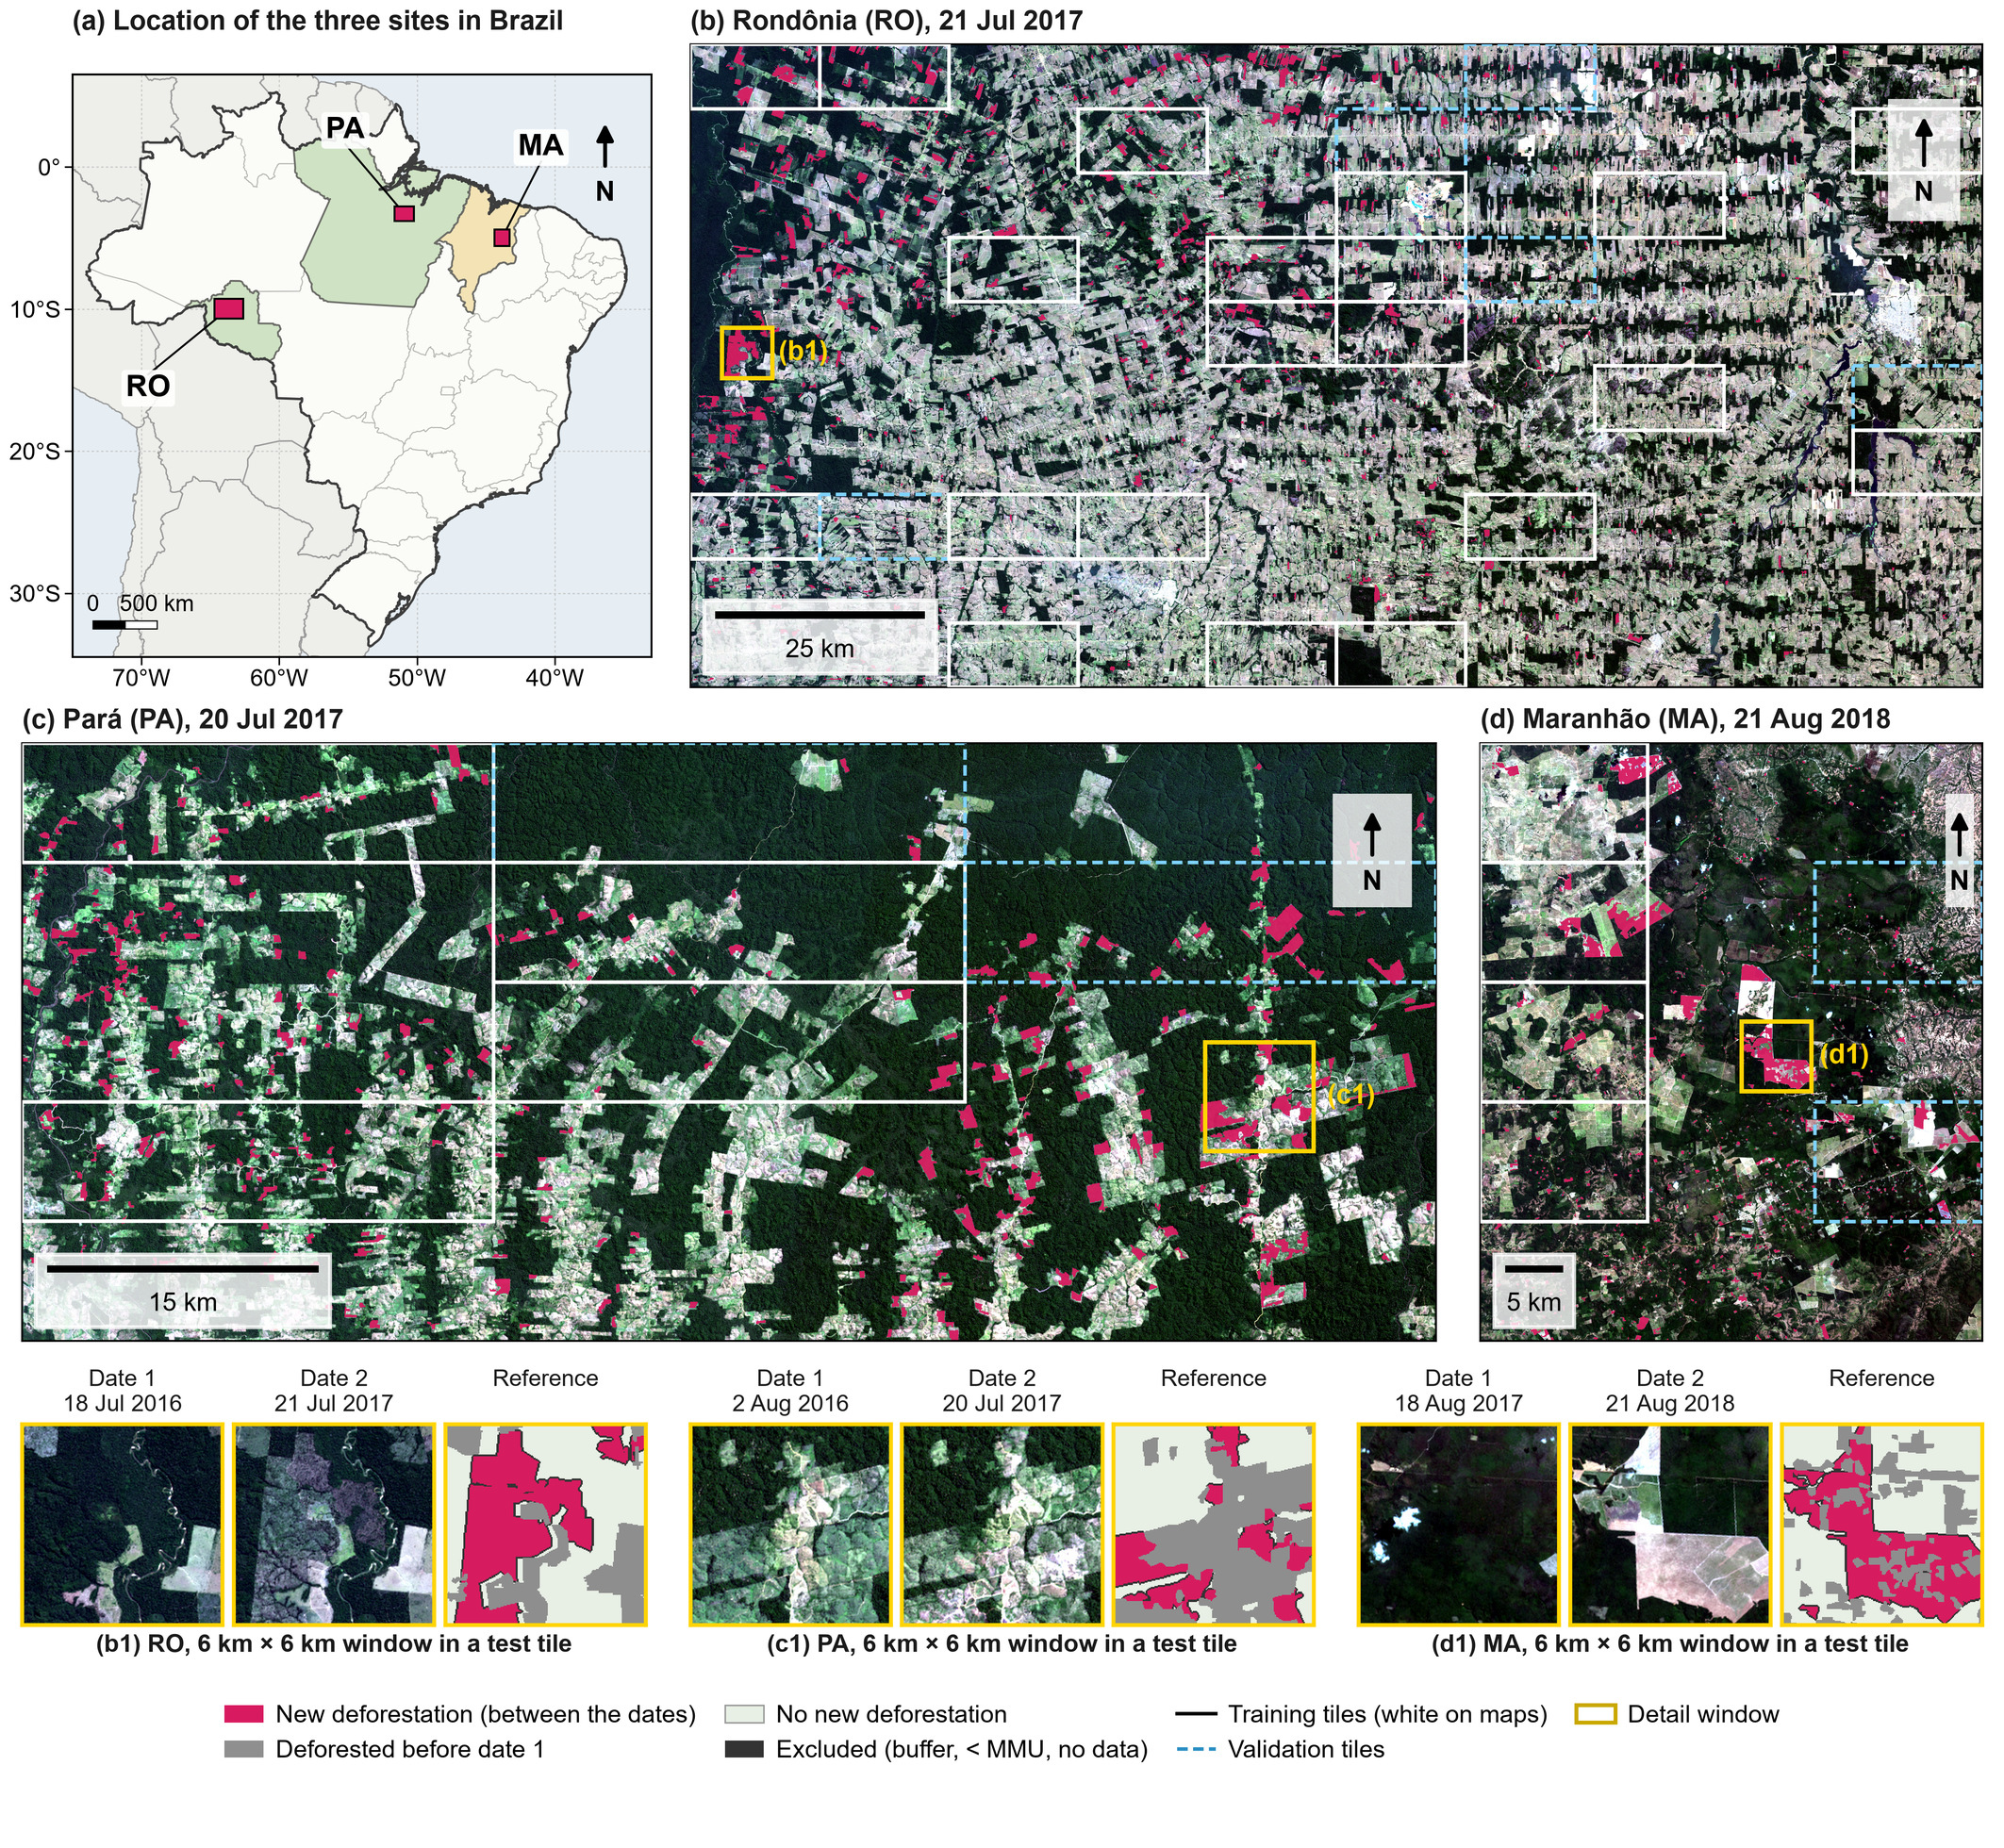
\includegraphics[width=\textwidth]{figures/ms/fig_study_area_code.jpg}
\caption{Study sites. (a) Location of the three Landsat-8 scenes (footprints from \citealp{noa2021adversarial}, Table~1; state outlines from Natural Earth). (b--d) Date-2 true-colour composites (OLI B4, B3, B2) of RO, PA and MA with the reference new deforestation, the training and validation tiles used in all experiments, and one detail window per site. (b1--d1) Detail windows ($6\times6$\,km, inside test tiles): date 1, date 2 and the reference, including the excluded pixels. Drawn in code from the study data.}
\label{fig:study_area}
\end{figure}

\textbf{Inputs.}
Each date is standardized per band over its whole scene (z-score), and the two dates are concatenated into a 14-band input.
No-data (NaN) pixels occur only in RO (\NoDataRO\% of the scene); they are filled with the band median before standardization and excluded from training and evaluation.

\textbf{Masks.}
Pixels are excluded (``void'') from loss and metrics if they carry no image data on either date, were deforested before the first date, lie in a 2-pixel ring around new-deforestation polygons, or belong to new-deforestation polygons smaller than the PRODES minimum mapping unit, i.e.\ 69 pixels (6.25\,ha) for PA and RO and 11 pixels (1\,ha) for MA.
These are the masking rules of the benchmark~\citep{demoura2025enhancing}.

\textbf{Splits.}
Each scene is cut into a grid of tiles, which are assigned to training, validation and test.
The tile counts follow the benchmark~\citep{noa2021adversarial,demoura2025enhancing}: RO uses a $10\times10$ grid with 20/5/75 tiles; PA and MA use 15 tiles each, split 4/2/9.
The benchmark fixes which tiles go to each split~\citep[Table~2]{demoura2025enhancing}.
We instead drew the assignment once at random (seed 42) and kept it fixed for every experiment, so our test regions differ from those of published results.
Our scene arrays are also slightly larger than the sizes reported for the benchmark (Table~\ref{tab:data}; 2550$\times$5120, 1098$\times$2600 and 1700$\times$1440 pixels for RO, PA and MA in \citealp{demoura2025enhancing}).
For these reasons, and because the networks differ, our absolute \Fone{} values should not be compared directly with published numbers; all comparisons in this paper are between methods evaluated on the same splits.
Training and validation patches ($64\times64$, stride 8) lie entirely inside tiles of their split and are kept only if at least 2\% of their valid pixels are new deforestation, following \citet{noa2021adversarial}.
Table~\ref{tab:data} lists the resulting sizes.

\begin{table}[htbp]
\centering
\caption{Data used in each site, as measured from the processed arrays.}
\label{tab:data}
% Generated by make_paper_numbers.py. Do not edit by hand.
\begin{tabular}{@{}lccc@{}}
\toprule
 & PA & RO & MA \\
\midrule
Scene size (px) & 1100$\times$2600 & 2554$\times$5130 & 1719$\times$1442 \\
Tile grid & 5$\times$3 & 10$\times$10 & 5$\times$3 \\
Tiles train/val/test & 4/2/9 & 20/5/75 & 4/2/9 \\
MMU (px) & 69 & 69 & 11 \\
Valid pixels (\%) & 67.2 & 30.2 & 58.7 \\
Deforestation (\% of valid) & 4.30 & 5.66 & 4.93 \\
Train / val patches & 3{,}167 / 1{,}090 & 8{,}487 / 2{,}188 & 3{,}375 / 1{,}578 \\
Test pixels (valid) & 1{,}077{,}074 & 3{,}007{,}586 & 1{,}043{,}263 \\
\bottomrule
\end{tabular}

\end{table}

% ============================================================
\section{Methods}\label{sec:methods}

Fig.~\ref{fig:method} summarizes the workflow, from the data to the evaluation.

\begin{figure}[tbp]
\centering
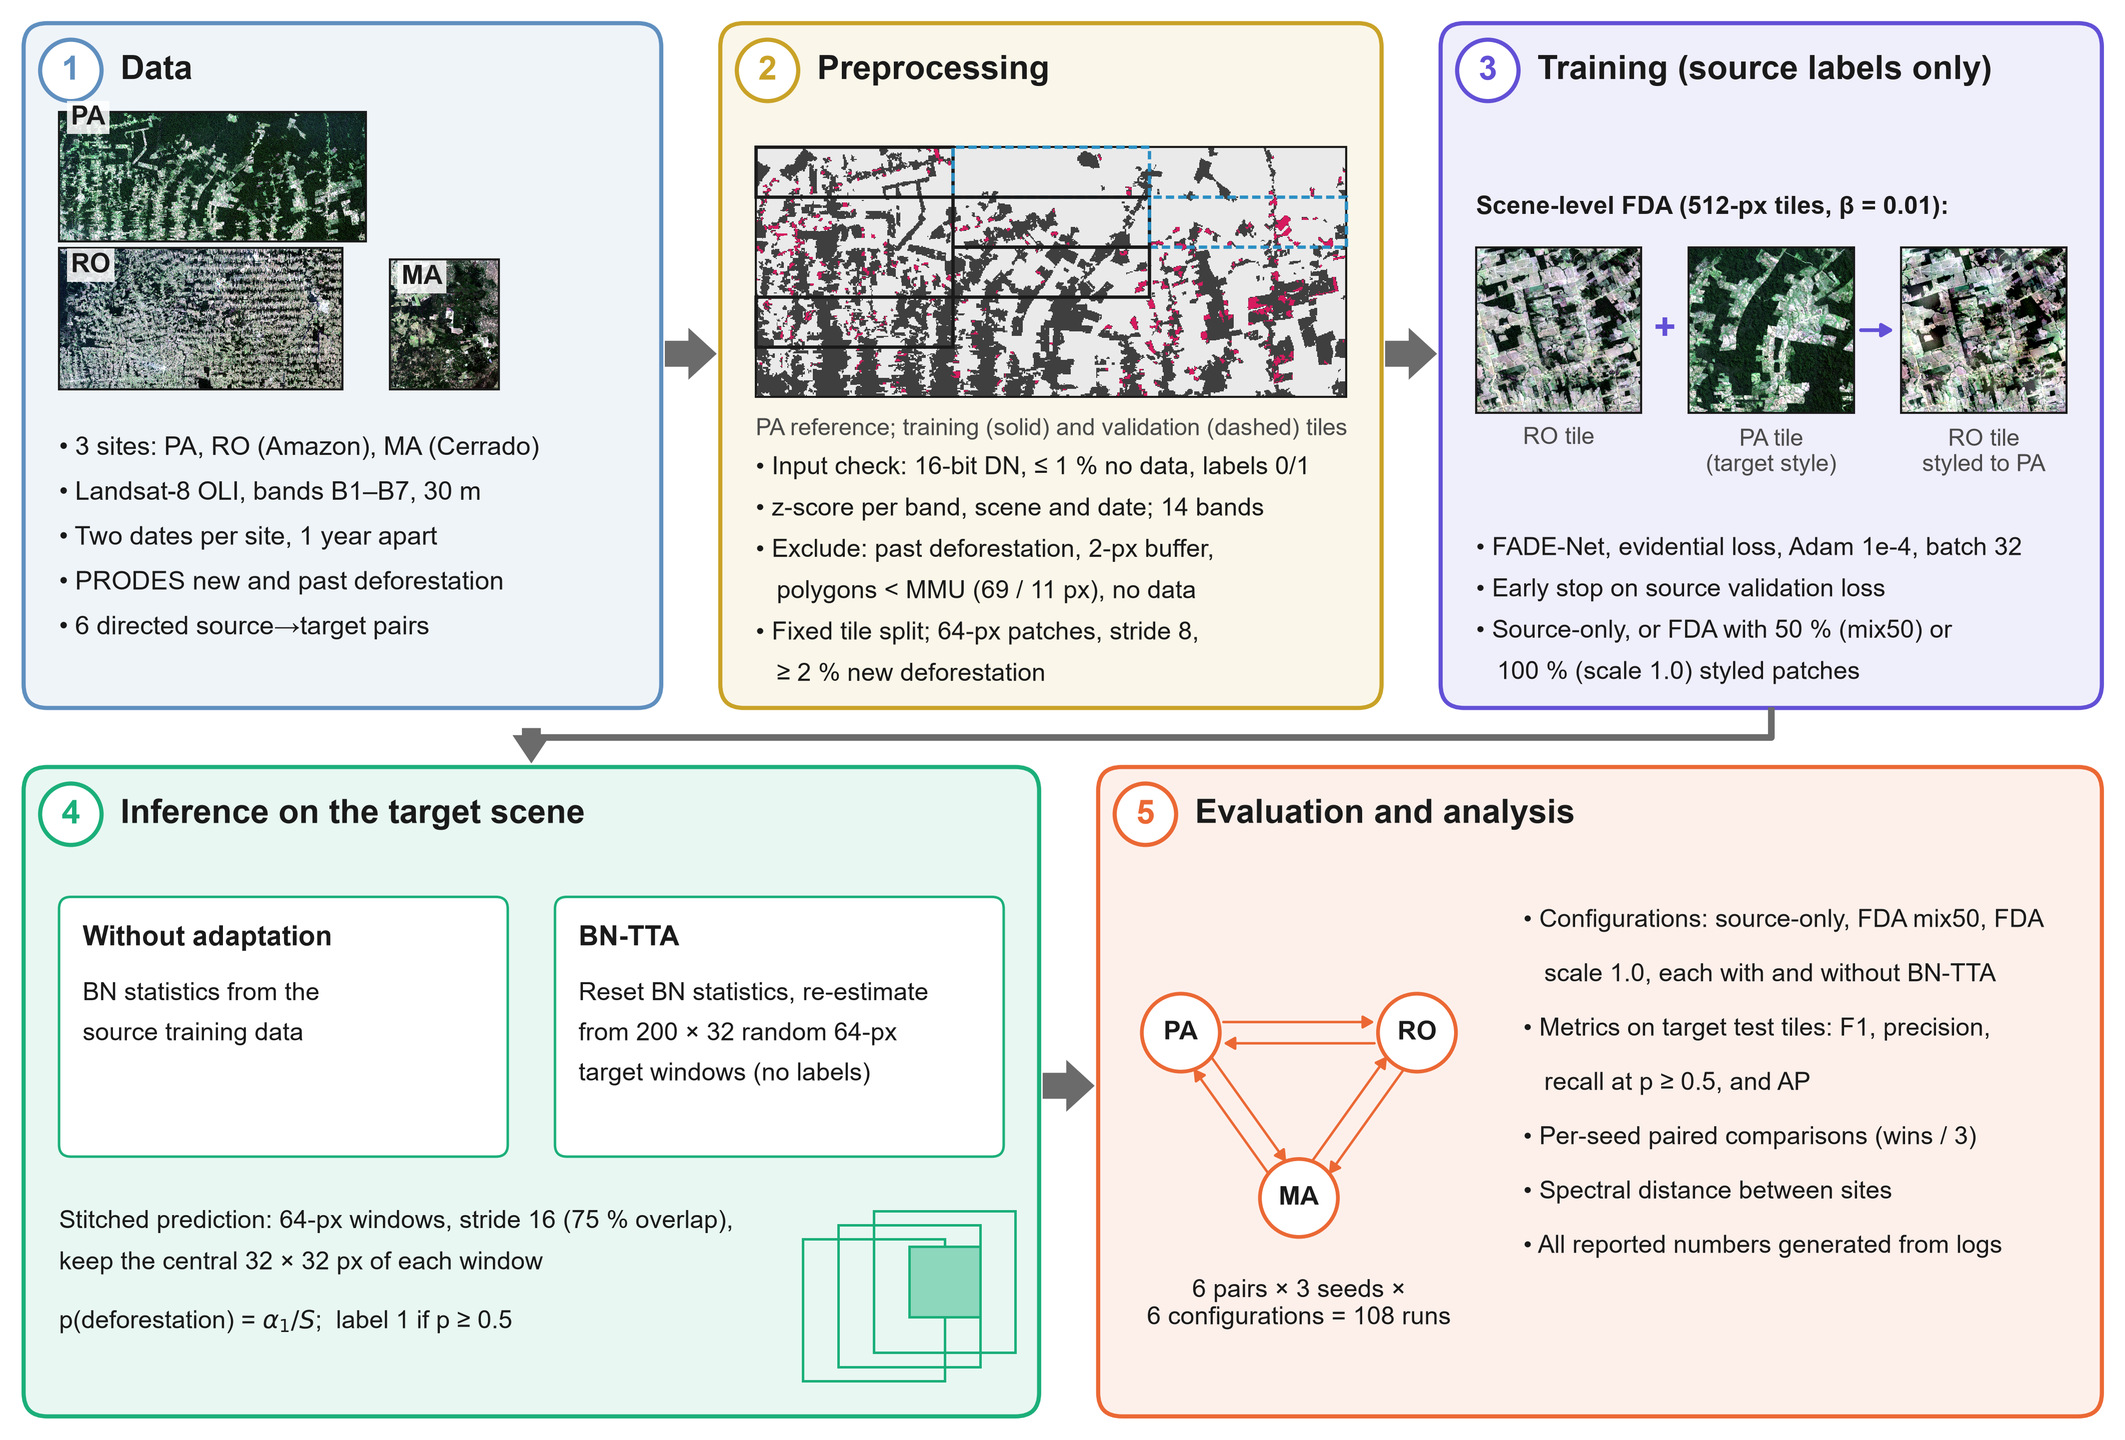
\includegraphics[width=\textwidth]{figures/ms/fig_methodology.jpg}
\caption{Overview of the study. Images are study data: date-2 scenes (1), the PA reference with the tile split (2), and a $512\times512$ RO tile before and after scene-level FDA toward PA (3).}
\label{fig:method}
\end{figure}

\subsection{Network and training}

The network (FADE-Net, \ParamsM{}\,M parameters) is a small encoder--decoder that outputs Dirichlet evidence~\citep{sensoy2018evidential}.
The encoder applies a $3\times3$ convolution ($14\to128$ channels), a stride-2 convolution to 256 channels ($32\times32$) and a stride-2 convolution to 512 channels ($16\times16$), each followed by BN and ReLU.
These are followed by two residual bottleneck blocks at $16\times16$.
The bottleneck was designed around a Mamba state-space block, but the \texttt{mamba\_ssm} package was not available in our environment, so every experiment used the implemented fallback: a ConvNeXt-style block ($7\times7$ depthwise convolution, BN, $1\times1$ expansion to $4\times$, GELU, $1\times1$ projection) with a residual connection inside the block and another in its wrapper, so that each block outputs $2x + f(x)$ (Fig.~\ref{fig:arch}).
The decoder upsamples with a transposed convolution to $32\times32$, fuses the result with the 256-channel encoder features ($3\times3$ convolution, BN, ReLU), upsamples to $64\times64$ and maps 128 channels to two classes with a $1\times1$ convolution and a softplus.
The softplus outputs are the evidence $e_k\ge0$ of a Dirichlet with $\alpha_k = e_k + 1$, and the predicted probability of deforestation is $\alpha_1/S$ with $S=\alpha_0+\alpha_1$.

\begin{figure}[htbp]
\centering
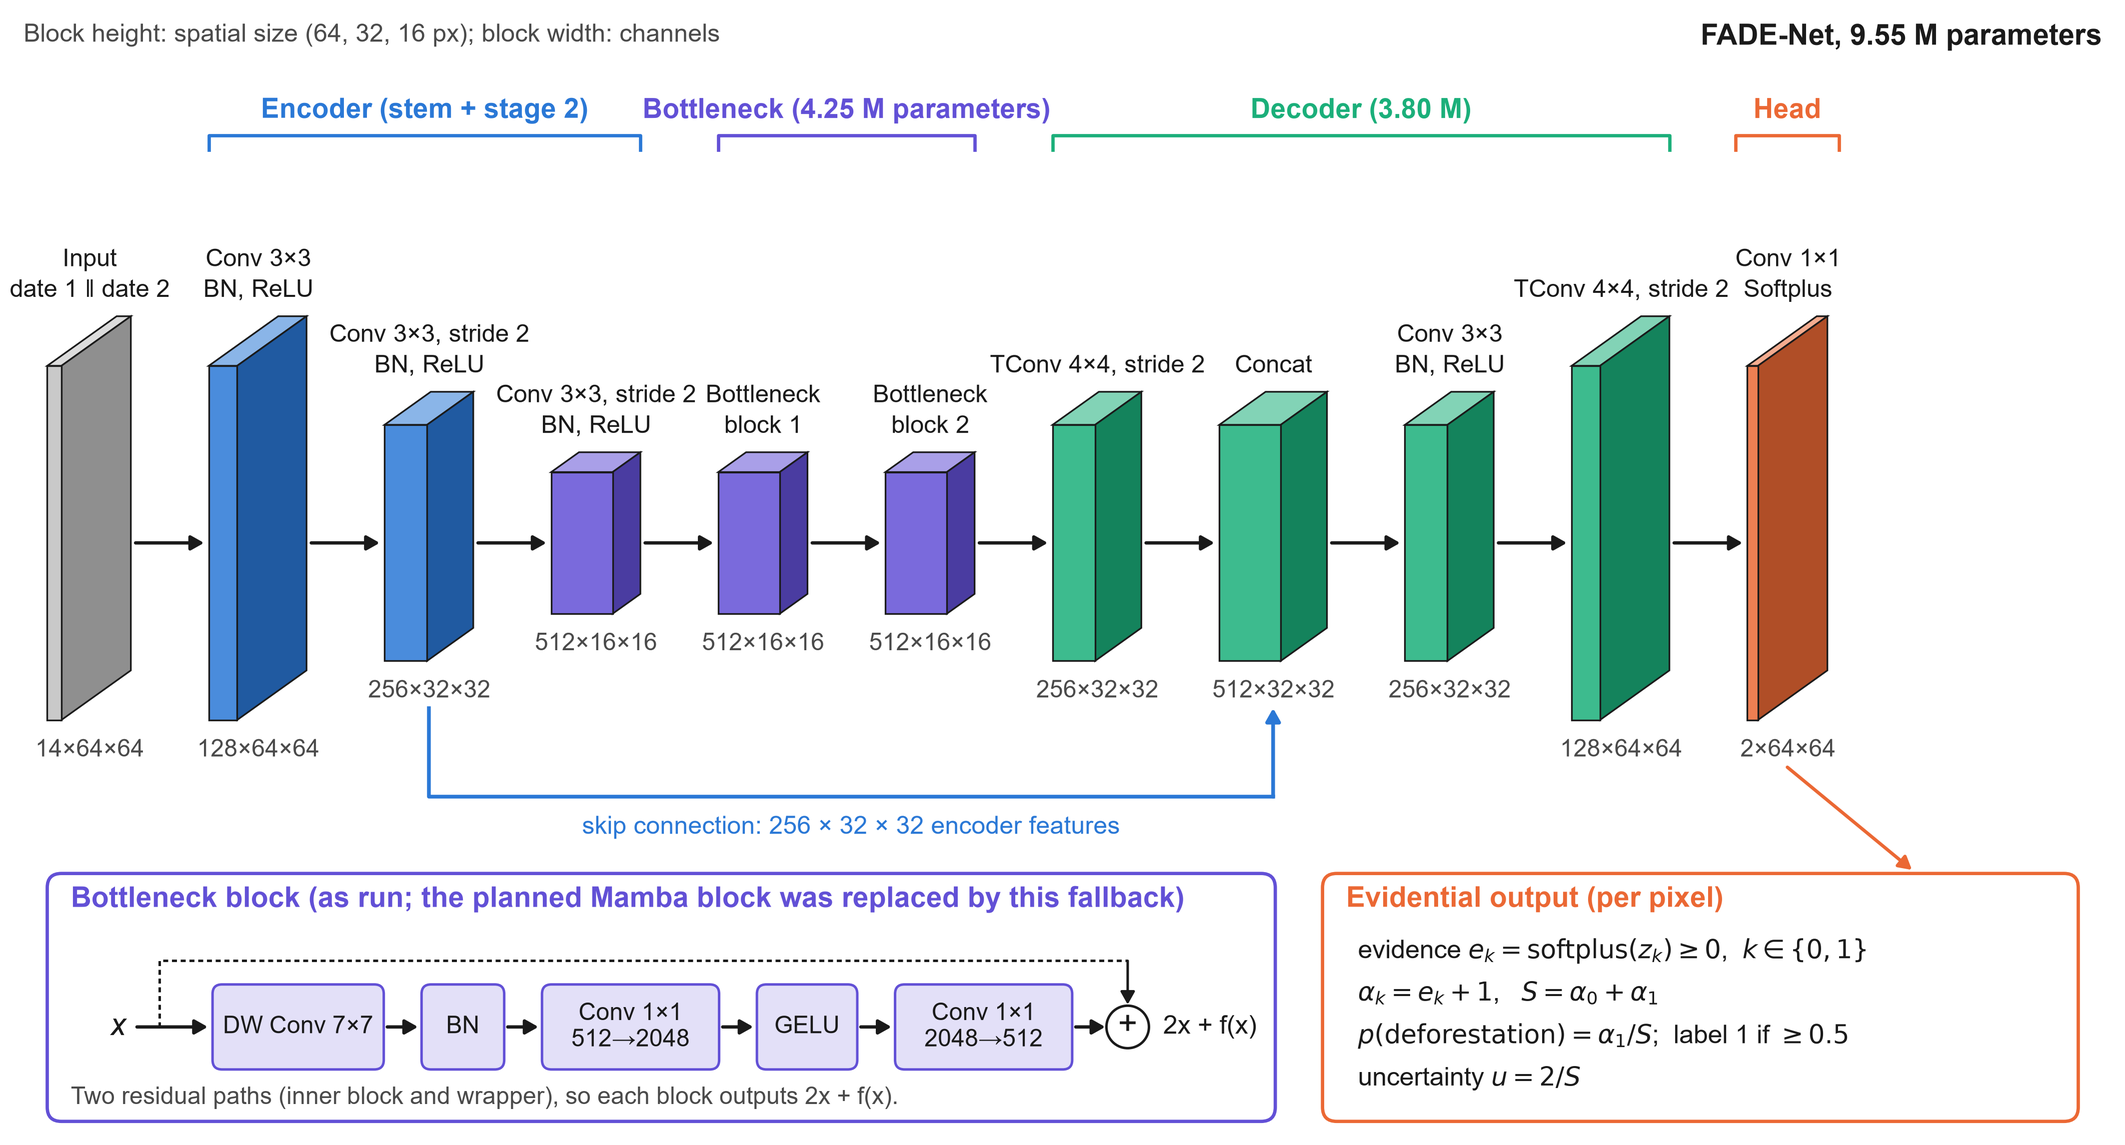
\includegraphics[width=\textwidth]{figures/ms/fig_architecture.png}
\caption{FADE-Net as used in all experiments, with tensor sizes for a $14\times64\times64$ input. Block height indicates spatial size and block width the number of channels. Parameter counts are measured from the implementation.}
\label{fig:arch}
\end{figure}

Training minimizes the evidential loss of \citet{sensoy2018evidential} on valid pixels:
\begin{equation}
\mathcal{L} = w_y \textstyle\sum_k y_k\bigl(\psi(S)-\psi(\alpha_k)\bigr) + \lambda_t\, w_y\, \mathrm{KL}\bigl(\mathrm{Dir}(\tilde\alpha)\,\|\,\mathrm{Dir}(\mathbf 1)\bigr),
\end{equation}
where $\psi$ is the digamma function, $\tilde\alpha = y + (1-y)\odot\alpha$, $\lambda_t=\min(1, t/10)$ at epoch $t$, and the class weights are $w=0.4$ (no change) and $2.0$ (deforestation), the values used by \citet{torres2021deforestation} and \citet{demoura2025enhancing}.
We use Adam (learning rate $10^{-4}$), batch size 32, mixed precision, random $90^\circ$ rotations and flips, and at most 100 epochs.
Training stops when the source validation loss has not improved for 10 epochs (after at least 5), and the checkpoint with the lowest source validation loss is kept.
No target labels are used for training or model selection; FDA (Section~\ref{sec:fda}) additionally uses unlabeled target images.

\textbf{Inference and metrics.}
Whole scenes are predicted with $64\times64$ windows at stride 16 (75\% overlap), keeping the central $32\times32$ pixels of each window.
A pixel is labeled deforestation if $\alpha_1/S\ge0.5$.
We report \Fone{}, precision and recall of the deforestation class at this threshold, and average precision (AP, threshold-free), all on valid pixels of the test tiles.

\subsection{Test-time BN adaptation (\BNTTA{})}\label{sec:bntta}

Starting from a trained source model, we reset every BN layer's running mean and variance, set its momentum to cumulative averaging, and run 200 forward passes in training mode on batches of 32 random $64\times64$ windows of the target scene, with no gradients.
The model is then evaluated in inference mode.
The windows are drawn uniformly over the whole target scene with a fixed random seed, so they cover the test tiles too; no labels are used.
This makes the procedure transductive, as is usual for test-time adaptation.

\subsection{Fourier Domain Adaptation (FDA)}\label{sec:fda}

For a source image $x_s$ and a target image $x_t$ of size $N\times N$, FDA replaces the centered low-frequency square of the source amplitude spectrum with the target's and keeps the source phase~\citep{yang2020fda}:
\begin{equation}
x_{s\to t} = \mathcal F^{-1}\bigl[\,M_b\odot|\mathcal F x_t| + (1-M_b)\odot|\mathcal F x_s|,\; \angle\mathcal F x_s\bigr],
\end{equation}
where $M_b$ selects the $2b\times2b$ frequencies around zero and $b=\lfloor\beta N\rfloor$.

\textbf{The patch-size pitfall.}
For $64\times64$ patches and $\beta=0.01$, $b=\lfloor0.64\rfloor=0$, so $M_b$ is empty and FDA returns the source image unchanged (Fig.~\ref{fig:fda}).
Any pipeline that applies FDA per training patch at this size and $\beta$ is training on unstyled data.
At $N=512$ the same $\beta$ gives $b=5$, a swap of \FDABinsFiveTwelve{} of \FDATotalFiveTwelve{} frequency bins (\FDASwapPct\%).

\begin{figure}[htbp]
\centering
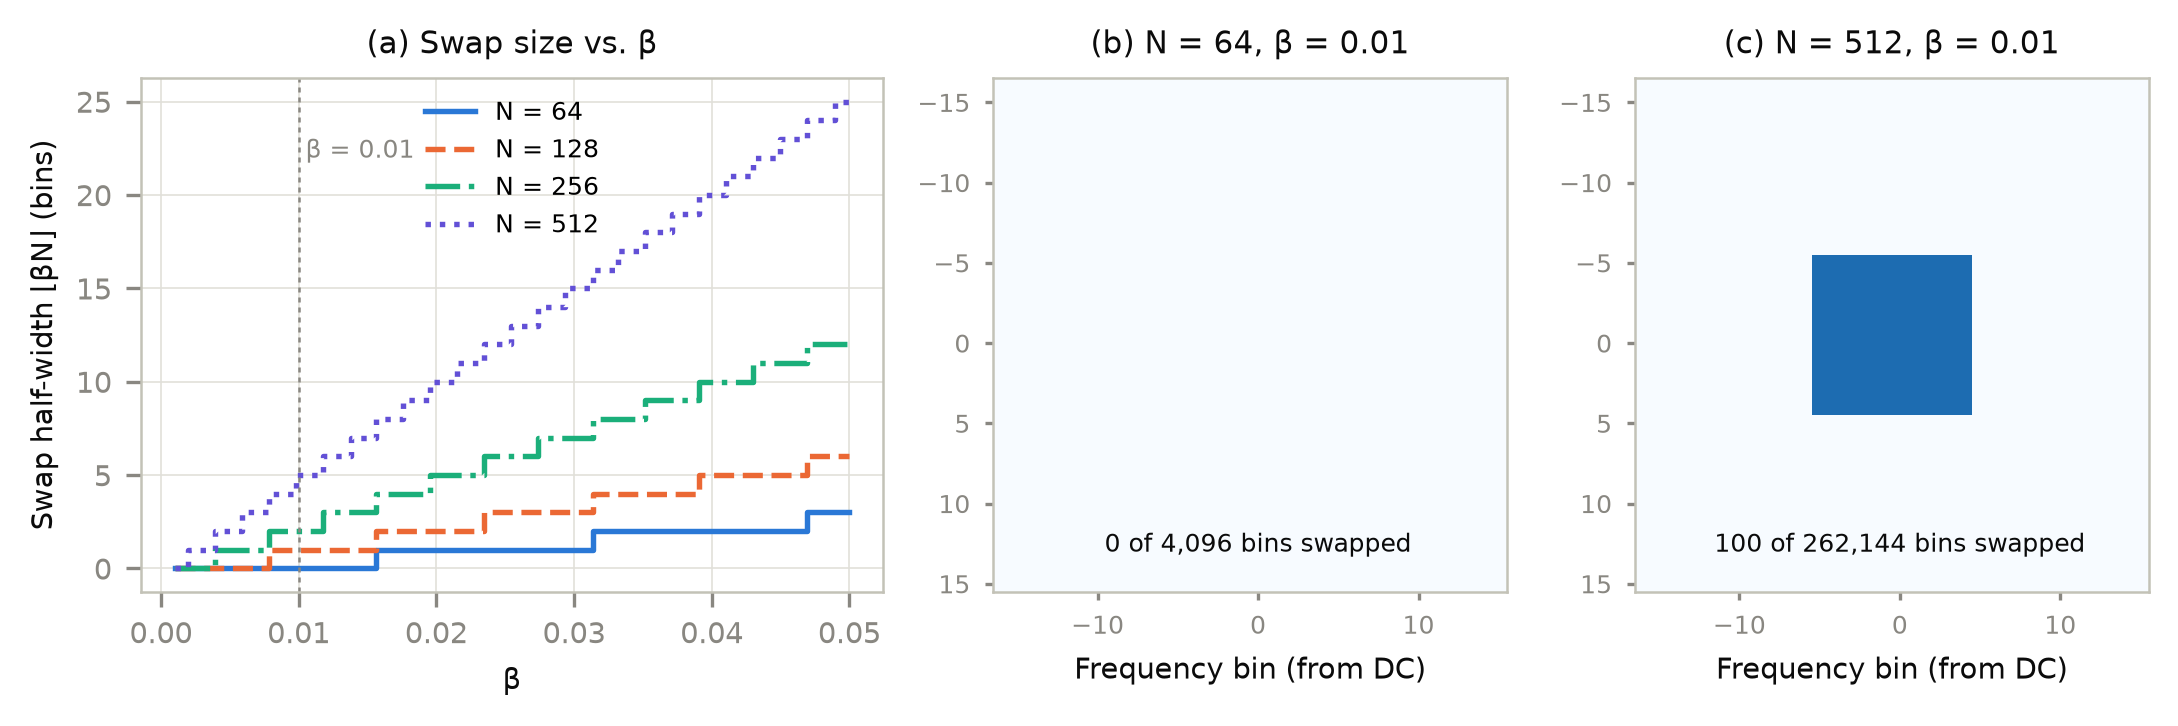
\includegraphics[width=0.9\textwidth]{figures/fig_fda_granularity.png}
\caption{FDA swap size. (a) Half-width $b=\lfloor\beta N\rfloor$ of the swapped square for four image sizes $N$. (b) At $N=64$ and $\beta=0.01$ no frequency is swapped. (c) At $N=512$ the same $\beta$ swaps a $10\times10$ square around zero frequency (central $32\times32$ bins shown).}
\label{fig:fda}
\end{figure}

\textbf{Scene-level FDA.}
We therefore style raw (unnormalized) source scenes tile by tile with $512\times512$ tiles.
Each tile receives the low-frequency amplitude of a random same-size crop of the target scene from the same acquisition date.
Edge tiles too thin for a non-empty swap ($\lfloor0.01h\rfloor<1$) are left unchanged: \FDAUnstyledPA{} of \FDATilesPA{} tiles in PA (\FDAUnstyledPctPA\% of pixels), \FDAUnstyledRO{} of \FDATilesRO{} in RO (\FDAUnstyledPctRO\%) and none in MA.
The styled scenes are then normalized and patched as in Section~\ref{sec:data}.
We build three styled versions of each source scene per target ($\beta=0.01$).
During training and validation, each patch is drawn from a random styled version with probability $s$ and from the original scene otherwise.
We test $s=0.5$ (``FDA mix50'') and $s=1.0$ (``FDA scale 1.0'').
Because validation patches are styled too, model selection for FDA runs uses a styled source validation set.

\subsection{Experimental design}



We evaluate six configurations on all six directional pairs: source-only, source-only + \BNTTA{}, FDA mix50, FDA mix50 + \BNTTA{}, FDA scale 1.0 and FDA scale 1.0 + \BNTTA{}.
Each configuration is trained with seeds 42, 123 and 456.
Training is deterministic: rerunning with the same source domain and seed reproduces the checkpoint exactly, so the source-only runs for the two targets of a source domain share one model.
The source-only results therefore come from 9 distinct models.
FDA models depend on the target and are trained per pair.
We report the mean and sample standard deviation over the three seeds.
For each adaptation method we also count the seeds in which it beats source-only with the same seed.
With three seeds we do not run significance tests; the counts and the per-seed points (Fig.~\ref{fig:seeds}) show how consistent each effect is.

\subsection{Implementation and use of AI tools}\label{sec:impl}

All experiments were run with PyTorch on one NVIDIA RTX~4050 laptop GPU (6\,GB memory).
Claude (Anthropic; Claude Opus~5.5 and earlier Claude models, used through Claude Code) was used to write and debug the data-checking, training, evaluation and plotting code, to search for and check literature and references, and to draft and edit the manuscript text.
The author reviewed the code and the text and is responsible for the whole content.
Every number reported in the text, tables and figures is generated by scripts from the logged per-run outputs and checked automatically against them, and every reference was checked against its publisher or Crossref record.
No generative AI tool was used to create or alter any image; all figures are drawn in code from the study data.

% ============================================================
\section{Results}\label{sec:results}

\subsection{In-domain accuracy and the transfer gap}

Fig.~\ref{fig:matrix} shows the source-only results.
In-domain test \Fone{} is \InDomPAM{} $\pm$ \InDomPAS{} for PA, \InDomROM{} $\pm$ \InDomROS{} for RO and \InDomMAM{} $\pm$ \InDomMAS{} for MA.
Across domains, \Fone{} falls to between \SOMin{} (\pr{PA}{RO}) and \SOMax{} (\pr{MA}{PA}).
Transfer is strongly directional.
A model trained on MA reaches \SOMAPAM{} on PA, close to a model trained on PA itself (\InDomPAM{}), whereas a model trained on PA reaches only \SOPAMAM{} on MA.
Similarly, \pr{MA}{RO} (\SOMAROM{}) transfers better than \pr{RO}{MA} (\SOROMAM{}).
RO is the hardest target from PA (\SOPAROM{}), although both sites are in the Amazon biome.
The same qualitative pattern appears in the source-only baselines of \citet{demoura2025enhancing}: transfer from MA to PA is the strongest of the six pairs and transfer from PA to RO the weakest. They attribute the good generalization of MA-trained models to the higher variability of MA's forest, following the class-complexity analysis of \citet{sotovega2021unsupervised}.

\begin{figure}[htbp]
\centering
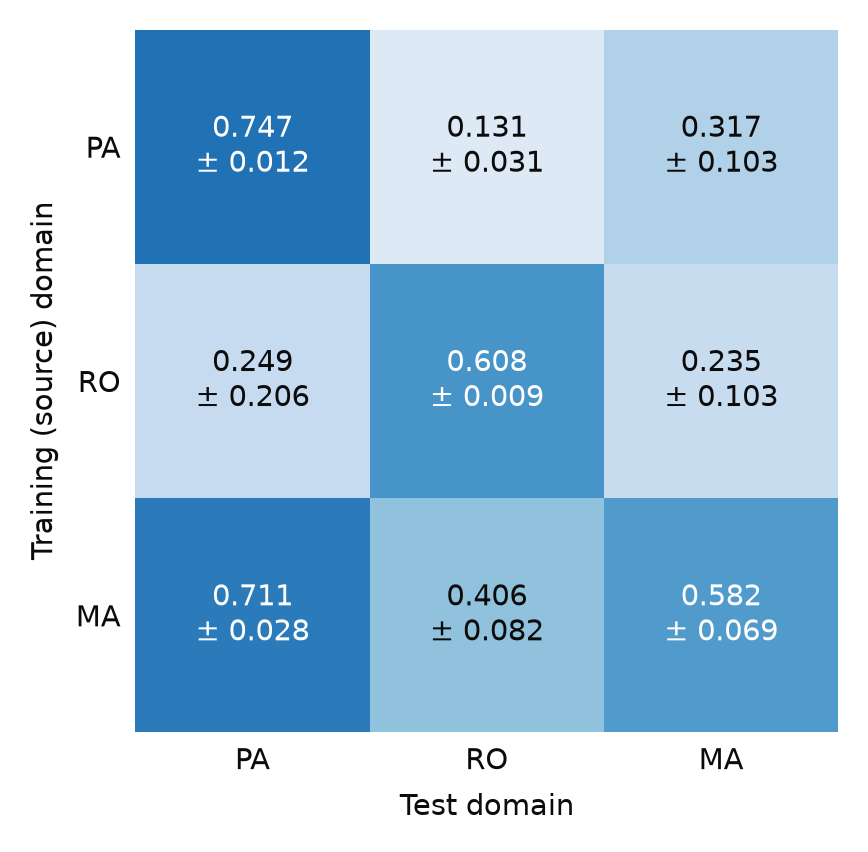
\includegraphics[width=0.5\textwidth]{figures/fig_transfer_matrix.png}
\caption{Source-only test \Fone{} (mean $\pm$ std over three seeds). Rows: training domain; columns: test domain. The diagonal is in-domain accuracy.}
\label{fig:matrix}
\end{figure}

\subsection{Seed variance}

The standard deviation of source-only target \Fone{} over three seeds ranges from \SOStdMin{} to \SOStdMax{} across pairs.
For \SOWidestPair{}, the three seeds give \Fone{} from \SOWidestLo{} to \SOWidestHi{}.
These seeds differ only in initialization and data order.
The spread is as large as most of the method differences below, so a single-seed comparison on this benchmark can easily rank methods wrongly.

\subsection{Test-time BN adaptation}

Table~\ref{tab:f1} and Fig.~\ref{fig:seeds} give target \Fone{}, and Table~\ref{tab:ap} gives AP.
\BNTTA{} raises \Fone{} in all three seeds for \pr{PA}{RO} (\TTAPAROD{} on average), \pr{RO}{MA} (\TTAROMAD{}) and \pr{PA}{MA} (\TTAPAMAD{}), and in two of three for \pr{RO}{PA} (\TTAROPAD{}).
It lowers \Fone{} for both pairs trained on MA: \pr{MA}{PA} drops in every seed (\TTAMAPAD{}) and \pr{MA}{RO} in two of three (\TTAMAROD{}).
Over all \TTAAllN{} paired runs the mean change is \TTAAllD{}.

AP shows a more consistent picture.
\BNTTA{} raises AP in \TTAAPAllW{} of \TTAAPAllN{} paired runs (mean \TTAAPAllD{}), including all three seeds of \pr{MA}{RO} (\TTAAPMAROD{}).
It leaves AP essentially unchanged for \pr{PA}{MA} (\TTAAPPAMAD{}) and lowers it for \pr{MA}{PA} (\TTAAPMAPAD{}).
On the MA-source pairs the \Fone{} loss therefore comes mainly from the operating point.
For \pr{MA}{RO}, mean recall rises from \SORMAROM{} to \TTARMAROM{} while precision falls from \SOPMAROM{} to \TTAPMAROM{}.
For \pr{MA}{PA}, recall rises from \SORMAPAM{} to \TTARMAPAM{} and precision falls from \SOPMAPAM{} to \TTAPMAPAM{}.
The re-estimated statistics move many more pixels above the fixed 0.5 threshold.
\BNTTA{} also lowers source-domain test \Fone{} by \TTASrcDropMean{} on average, as expected once the statistics no longer match the source.

The four pairs where \BNTTA{} raises \Fone{} are also the four with the lowest source-only \Fone{}, and the two where it lowers \Fone{} are the two highest.
Because the two highest are exactly the MA-source pairs, our data cannot separate ``MA as source'' from ``already high baseline'' as the explanation.

\begin{sidewaystable}
\centering
\caption{Target-domain test \Fone{} (mean $\pm$ std over seeds 42, 123, 456). In parentheses: number of seeds in which the method beats source-only with the same seed. Bold: best mean per pair.}
\label{tab:f1}
\footnotesize\setlength{\tabcolsep}{4pt}% Generated by make_paper_numbers.py. Do not edit by hand.
\begin{tabular}{@{}lcccccc@{}}
\toprule
Method & PA$\to$RO & RO$\to$PA & MA$\to$RO & RO$\to$MA & PA$\to$MA & MA$\to$PA \\
\midrule
Source-only & 0.131$\pm$0.031 & 0.249$\pm$0.206 & \textbf{0.406$\pm$0.082} & 0.235$\pm$0.103 & 0.317$\pm$0.103 & \textbf{0.711$\pm$0.028} \\
+ BN-TTA & 0.180$\pm$0.046 (3/3) & 0.307$\pm$0.056 (2/3) & 0.351$\pm$0.011 (1/3) & 0.291$\pm$0.070 (3/3) & \textbf{0.390$\pm$0.093} (3/3) & 0.555$\pm$0.095 (0/3) \\
\midrule
FDA mix50 & 0.145$\pm$0.025 (1/3) & 0.537$\pm$0.014 (3/3) & 0.208$\pm$0.044 (0/3) & \textbf{0.376$\pm$0.043} (2/3) & 0.343$\pm$0.101 (1/3) & 0.699$\pm$0.005 (1/3) \\
FDA mix50 + BN-TTA & 0.181$\pm$0.029 (3/3) & 0.360$\pm$0.029 (2/3) & 0.257$\pm$0.013 (0/3) & 0.270$\pm$0.025 (2/3) & 0.359$\pm$0.084 (2/3) & 0.561$\pm$0.047 (0/3) \\
FDA scale 1.0 & 0.191$\pm$0.032 (3/3) & \textbf{0.551$\pm$0.021} (3/3) & 0.239$\pm$0.012 (0/3) & 0.328$\pm$0.051 (2/3) & 0.274$\pm$0.000 (2/3) & 0.686$\pm$0.020 (1/3) \\
FDA scale 1.0 + BN-TTA & \textbf{0.201$\pm$0.033} (3/3) & 0.334$\pm$0.061 (2/3) & 0.280$\pm$0.022 (0/3) & 0.239$\pm$0.022 (2/3) & 0.274$\pm$0.031 (2/3) & 0.470$\pm$0.058 (0/3) \\
\bottomrule
\end{tabular}

\end{sidewaystable}

\begin{sidewaystable}
\centering
\caption{Target-domain test average precision (AP), same layout as Table~\ref{tab:f1}.}
\label{tab:ap}
\footnotesize\setlength{\tabcolsep}{4pt}% Generated by make_paper_numbers.py. Do not edit by hand.
\begin{tabular}{@{}lcccccc@{}}
\toprule
Method & PA$\to$RO & RO$\to$PA & MA$\to$RO & RO$\to$MA & PA$\to$MA & MA$\to$PA \\
\midrule
Source-only & 0.107$\pm$0.018 & 0.286$\pm$0.205 & 0.393$\pm$0.065 & 0.395$\pm$0.143 & 0.742$\pm$0.015 & \textbf{0.801$\pm$0.017} \\
+ BN-TTA & 0.152$\pm$0.042 (3/3) & 0.515$\pm$0.072 (3/3) & \textbf{0.524$\pm$0.036} (3/3) & \textbf{0.484$\pm$0.108} (3/3) & \textbf{0.742$\pm$0.010} (2/3) & 0.769$\pm$0.049 (0/3) \\
\midrule
FDA mix50 & 0.116$\pm$0.028 (1/3) & 0.626$\pm$0.048 (3/3) & 0.160$\pm$0.022 (0/3) & 0.370$\pm$0.054 (2/3) & 0.595$\pm$0.044 (0/3) & 0.791$\pm$0.001 (1/3) \\
FDA mix50 + BN-TTA & 0.154$\pm$0.040 (3/3) & \textbf{0.636$\pm$0.031} (3/3) & 0.232$\pm$0.008 (0/3) & 0.404$\pm$0.102 (2/3) & 0.597$\pm$0.048 (0/3) & 0.778$\pm$0.025 (1/3) \\
FDA scale 1.0 & 0.141$\pm$0.020 (3/3) & 0.614$\pm$0.021 (3/3) & 0.169$\pm$0.018 (0/3) & 0.378$\pm$0.044 (2/3) & 0.527$\pm$0.039 (0/3) & 0.773$\pm$0.019 (0/3) \\
FDA scale 1.0 + BN-TTA & \textbf{0.163$\pm$0.019} (3/3) & 0.586$\pm$0.027 (3/3) & 0.241$\pm$0.041 (0/3) & 0.348$\pm$0.039 (1/3) & 0.503$\pm$0.043 (0/3) & 0.729$\pm$0.037 (0/3) \\
\bottomrule
\end{tabular}

\end{sidewaystable}

\begin{figure}[htbp]
\centering
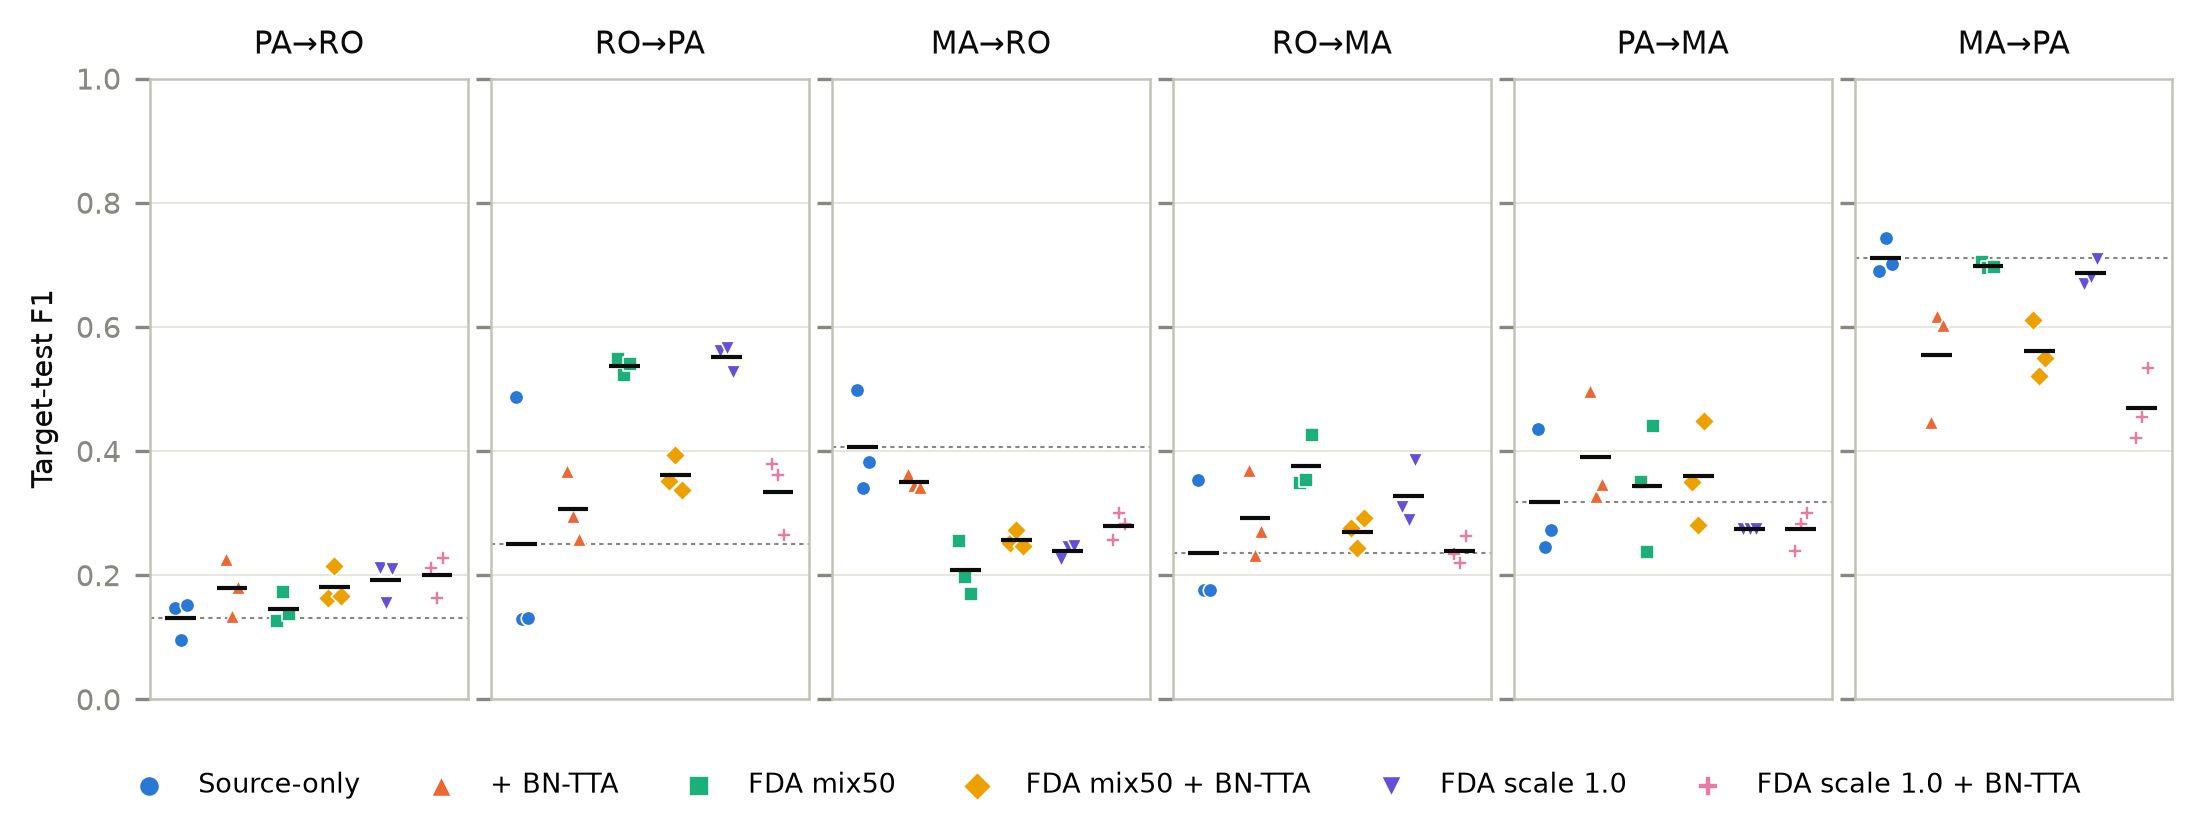
\includegraphics[width=\textwidth]{figures/fig_method_seeds.png}
\caption{Target-domain \Fone{} per seed (markers) and mean (black tick) for each method and pair. The dashed line is the source-only mean.}
\label{fig:seeds}
\end{figure}

\subsection{Fourier Domain Adaptation}

Over all \MIXAllN{} paired runs, FDA mix50 beats source-only \Fone{} in \MIXAllW{} (mean \MIXAllD{}) and FDA scale 1.0 in \ONEAllW{} (mean \ONEAllD{}).
These averages hide a clear dependence on the training domain:
\begin{itemize}[leftmargin=*, topsep=2pt, itemsep=1pt]
\item \textbf{RO as source:} FDA raises \Fone{} in \MIXSrcROW{}/\MIXSrcRON{} paired runs with mix50 (mean \MIXSrcROD{}) and \ONESrcROW{}/\ONESrcRON{} with scale 1.0 (\ONESrcROD{}). On \pr{RO}{PA} it also removes most of the seed spread: source-only gives \SOROPAM{} $\pm$ \SOROPAS{}, FDA mix50 \MIXROPAM{} $\pm$ \MIXROPAS{} and FDA scale 1.0 \ONEROPAM{} $\pm$ \ONEROPAS{}.
\item \textbf{PA as source:} the effect is small, \MIXSrcPAD{} (mix50, \MIXSrcPAW{}/\MIXSrcPAN{} wins) and \ONESrcPAD{} (scale 1.0, \ONESrcPAW{}/\ONESrcPAN{}).
\item \textbf{MA as source:} FDA lowers \Fone{} (mix50 \MIXSrcMAD{}, \MIXSrcMAW{}/\MIXSrcMAN{} wins; scale 1.0 \ONESrcMAD{}, \ONESrcMAW{}/\ONESrcMAN{}), most strongly on \pr{MA}{RO} in every seed.
\end{itemize}
AP follows the same split but is less favourable overall: FDA raises AP for RO-source pairs (mix50 \MIXAPSrcROD{}, scale 1.0 \ONEAPSrcROD{}) and lowers it for PA- and MA-source pairs, for an overall mean of \MIXAPAllD{} (mix50) and \ONEAPAllD{} (scale 1.0).

\textbf{Mixing ratio.}
Training on fully styled data (scale 1.0) and on a 50\% mix give similar results: scale 1.0 beats mix50 in \ONEvsMIXW{} of \ONEvsMIXN{} paired runs, with mean \Fone{} difference \ONEvsMIXD{}.
Fully styled training does not cause a collapse on clean test images in any pair.
On \pr{PA}{MA}, FDA scale 1.0 gives almost the same \Fone{} for all three seeds (range \ONEPAMAFRange{}).
This is a coincidence of the operating point: the three models differ in AP (\ONEPAMAAPLo{}--\ONEPAMAAPHi{}), precision, recall and training curves.

\textbf{FDA combined with \BNTTA{}.}
Adding \BNTTA{} to an FDA-trained model lowers \Fone{} relative to FDA alone in most paired runs (mix50: higher in only \MIXTTAvsMIXW{}/\MIXTTAvsMIXN{}, mean \MIXTTAvsMIXD{}; scale 1.0: \ONETTAvsONEW{}/\ONETTAvsONEN{}, mean \ONETTAvsONED{}).
For mix50 it still raises AP in \MIXTTAvsMIXAPW{}/\MIXTTAvsMIXAPN{} paired runs (mean \MIXTTAvsMIXAPD{}), the same threshold effect as for source-only models.

\textbf{What the methods change on the map.}
Fig.~\ref{fig:qual} shows predictions in one PA test window for the seed with the median effect of each method.
For \pr{MA}{PA}, \BNTTA{} turns most missed deforestation into detections but adds false alarms along the edges of cleared areas, which is the recall--precision trade described above.
For \pr{RO}{PA}, FDA removes most of the scattered false alarms of the source-only model, while most of the missed deforestation remains missed; in this example the \Fone{} gain comes from higher precision.

\begin{figure}[htbp]
\centering
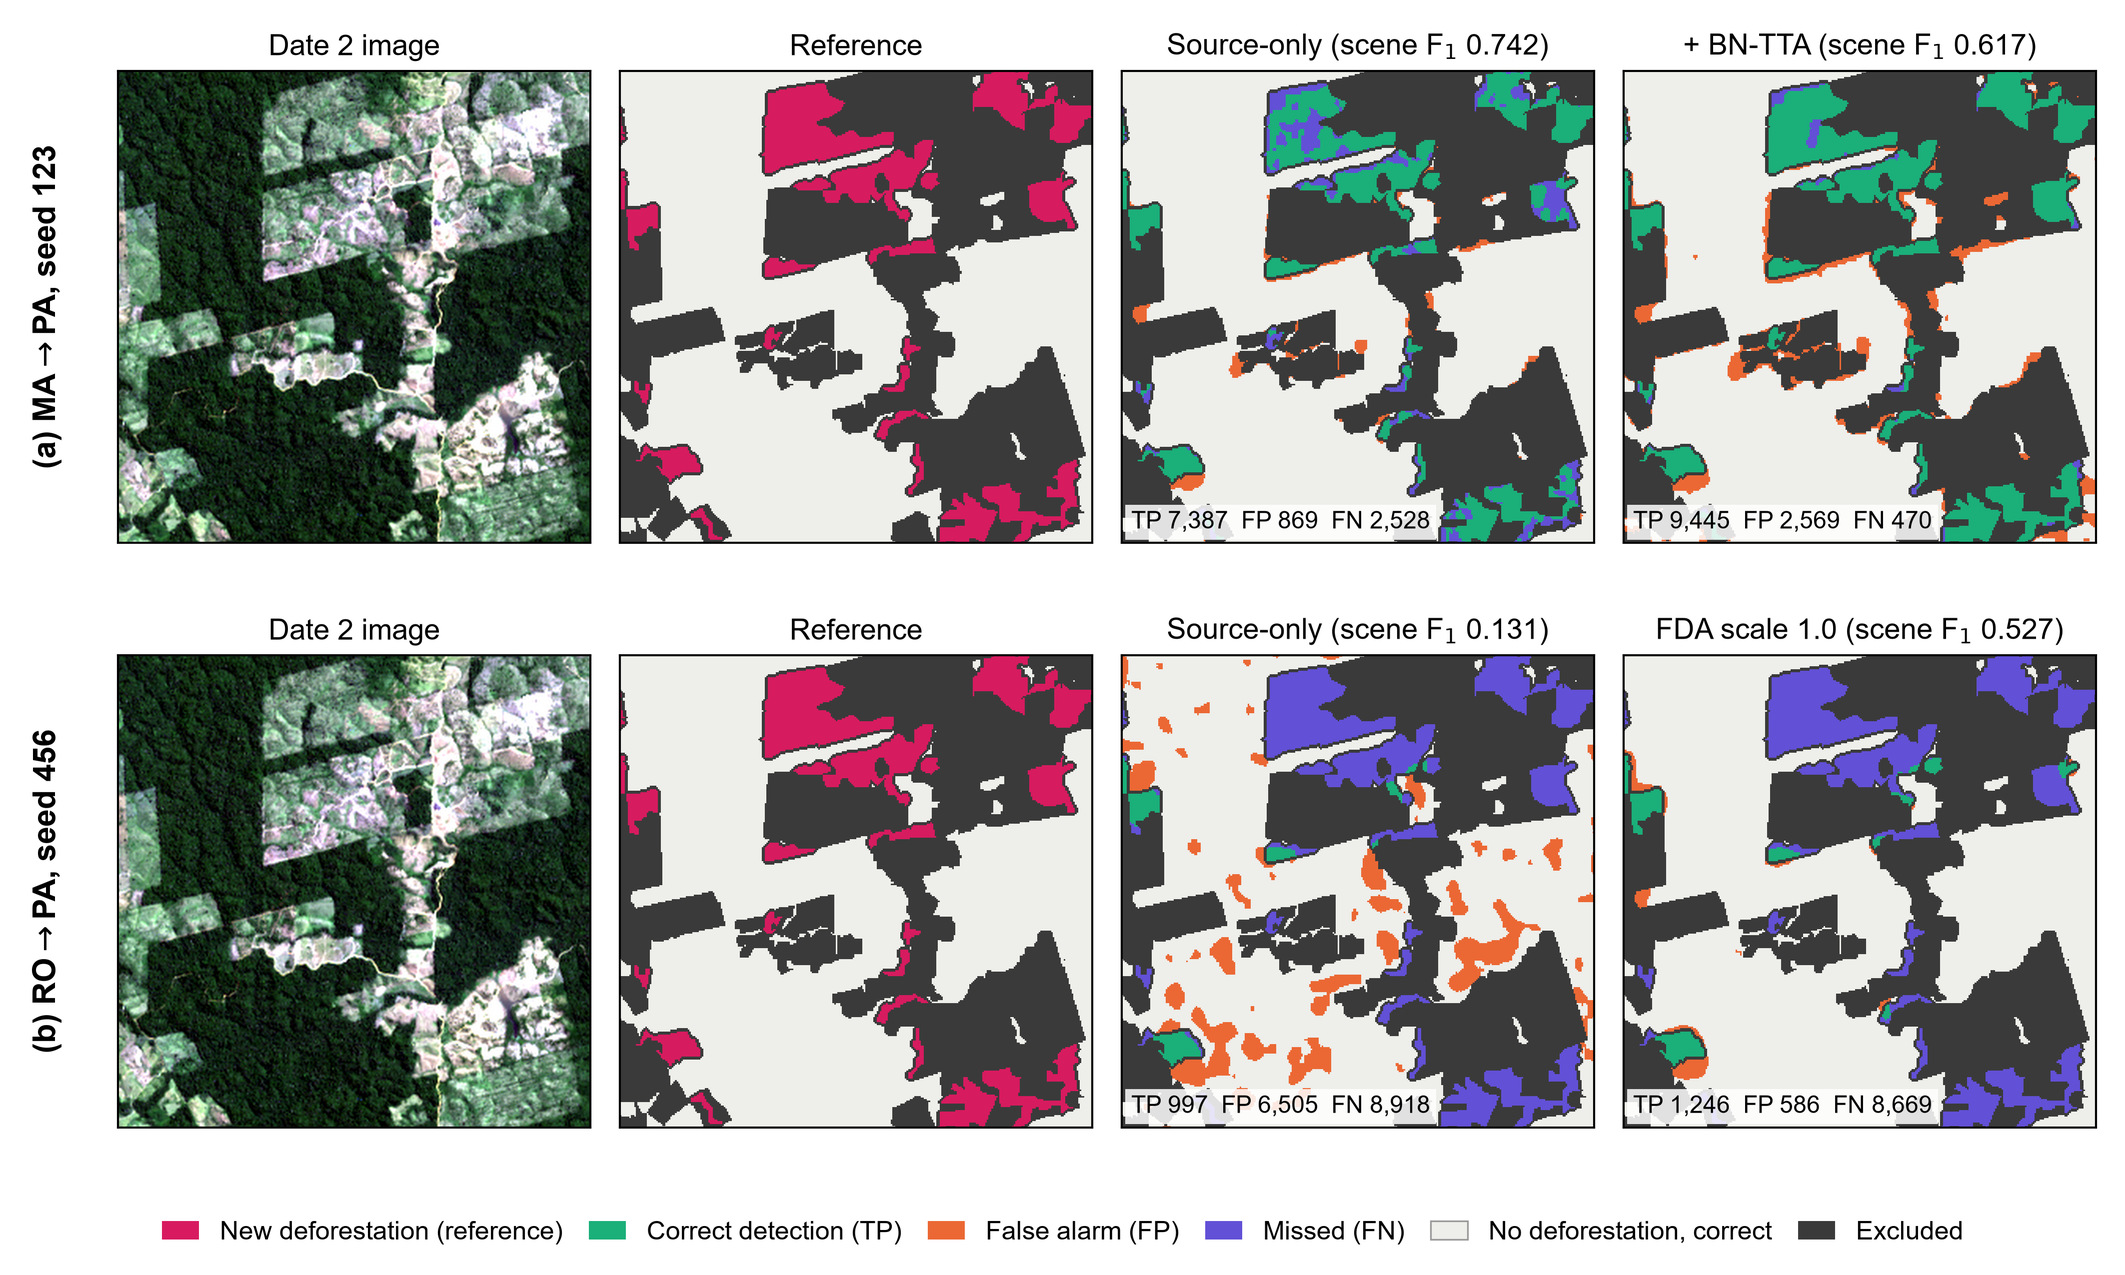
\includegraphics[width=\textwidth]{figures/ms/fig_qualitative.jpg}
\caption{Predictions in a $9\times9$\,km PA test window (the window with the most new deforestation inside test tiles). (a) \pr{MA}{PA} without and with \BNTTA{}; (b) \pr{RO}{PA} without and with FDA scale 1.0. For each pair, the seed is the one with the median \Fone{} change of the three seeds. Counts are pixels in the window; scene \Fone{} values are for all PA test tiles.}
\label{fig:qual}
\end{figure}

\textbf{No single best method.}
The configuration with the highest mean \Fone{} differs by pair: \BestPARO{} for \pr{PA}{RO}, \BestROPA{} for \pr{RO}{PA}, \BestROMA{} for \pr{RO}{MA}, \BestPAMA{} for \pr{PA}{MA}, and source-only for both MA-source pairs.

\subsection{Spectral distance between sites}

To check whether simple input statistics predict transfer difficulty, we computed radially averaged log-amplitude spectra of 20 random $512\times512$ tiles per scene and date, for each band (Fig.~\ref{fig:spectra}).
We define the distance between two sites as the mean absolute difference of their mean spectra, averaged over bands and dates.
On raw DNs, the distances are \SpecRawPARO{} (PA--RO), \SpecRawPAMA{} (PA--MA) and \SpecRawROMA{} (RO--MA).
On the per-scene normalized inputs the network actually receives, they are \SpecNormPARO{}, \SpecNormPAMA{} and \SpecNormROMA{} (Fig.~\ref{fig:distance}).
After normalization, PA and RO are the closest pair, and the clearest difference is MA's higher low-frequency amplitude in the NIR band.
Yet \pr{PA}{RO} is the hardest transfer in our results.
More generally, such distances are symmetric while the observed transfer is strongly directional, so on their own they cannot explain the transfer matrix.
With three sites this is a description, not a correlation analysis.

\begin{figure}[htbp]
\centering
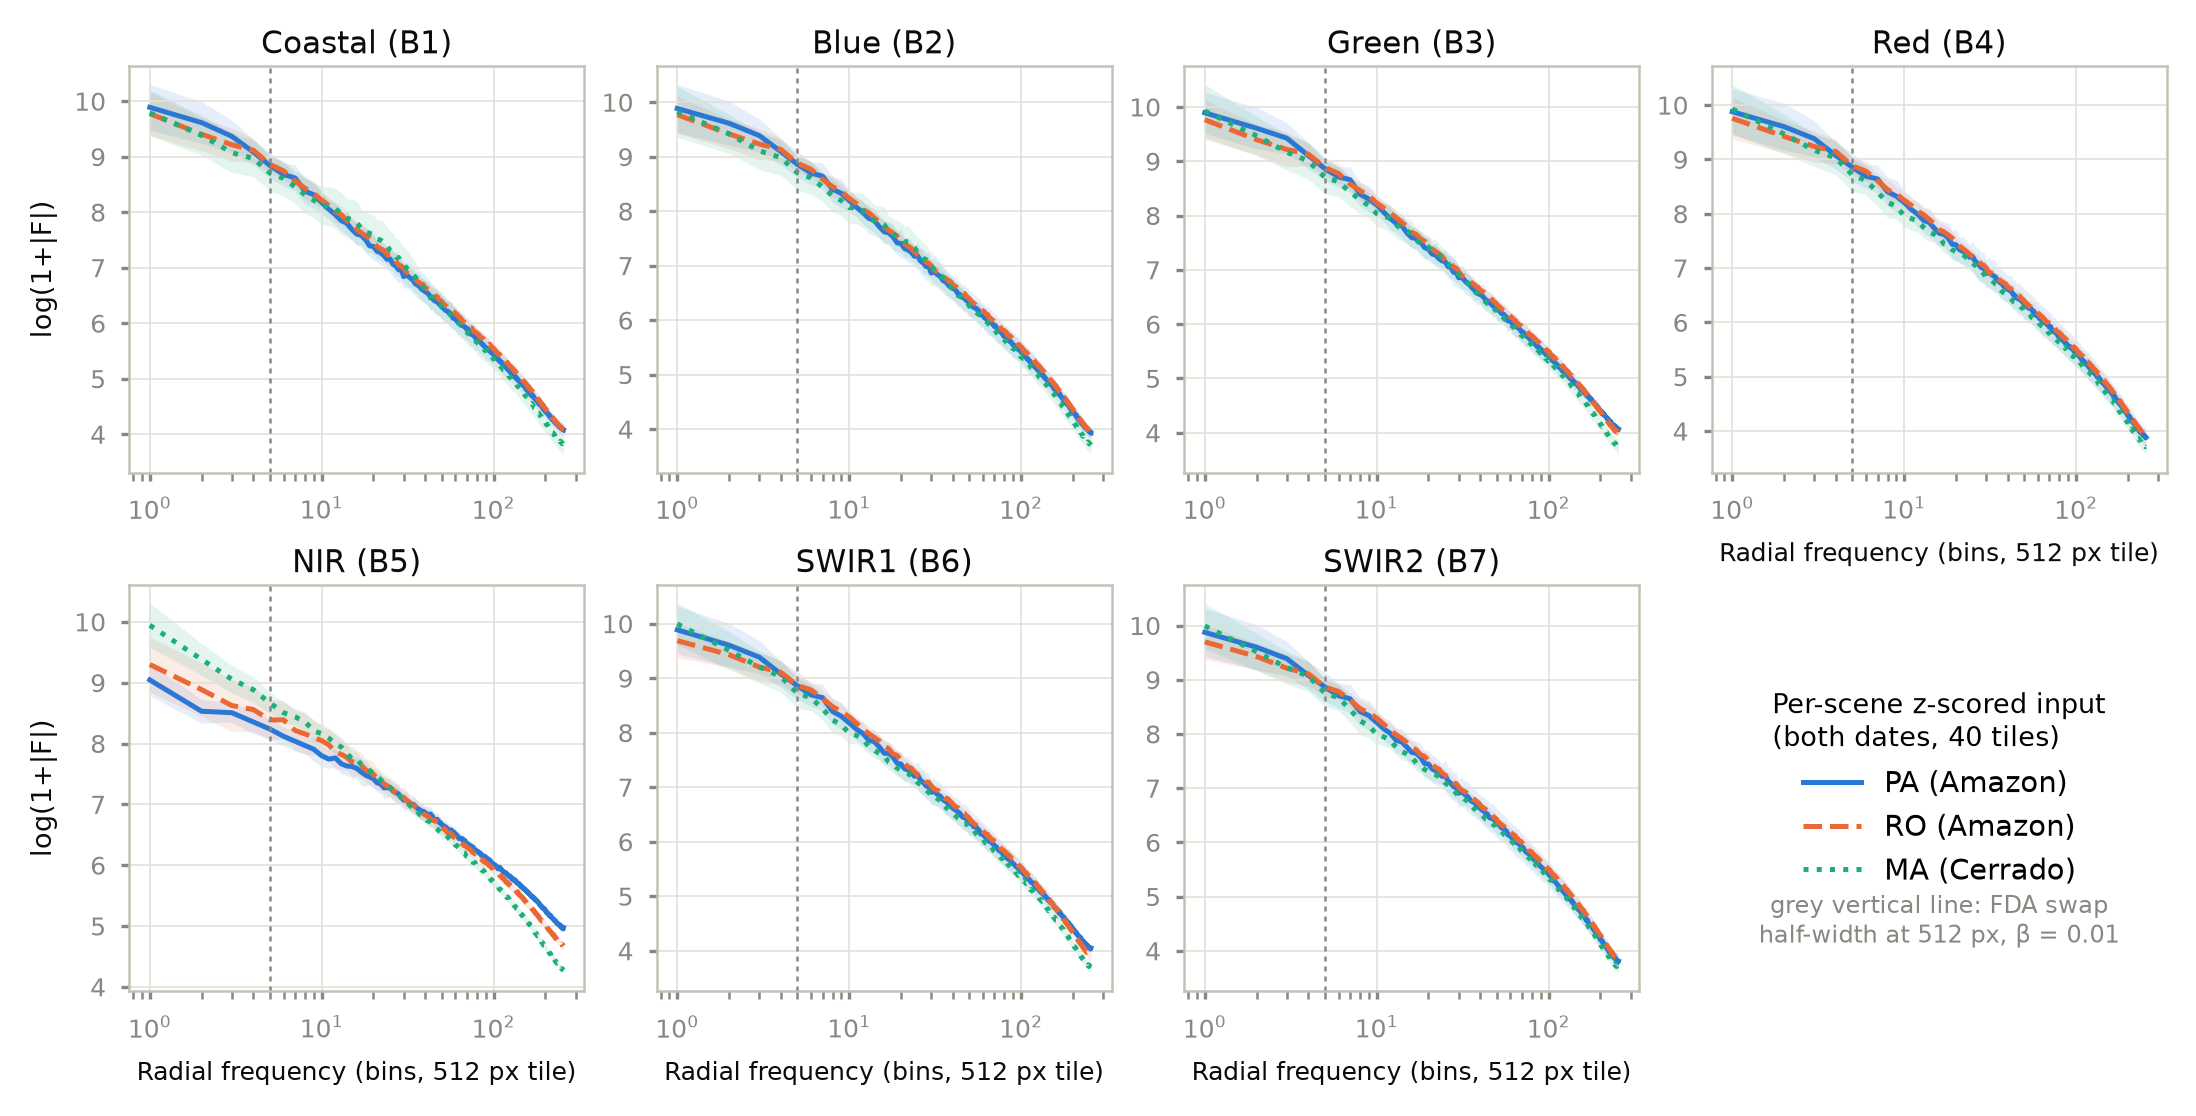
\includegraphics[width=\textwidth]{figures/fig_spectral_profiles.png}
\caption{Radially averaged log-amplitude spectra of the normalized inputs per band (mean $\pm$ std over 40 tiles: 20 per date). The grey vertical line marks the FDA swap half-width at $N=512$, $\beta=0.01$.}
\label{fig:spectra}
\end{figure}

\begin{figure}[htbp]
\centering
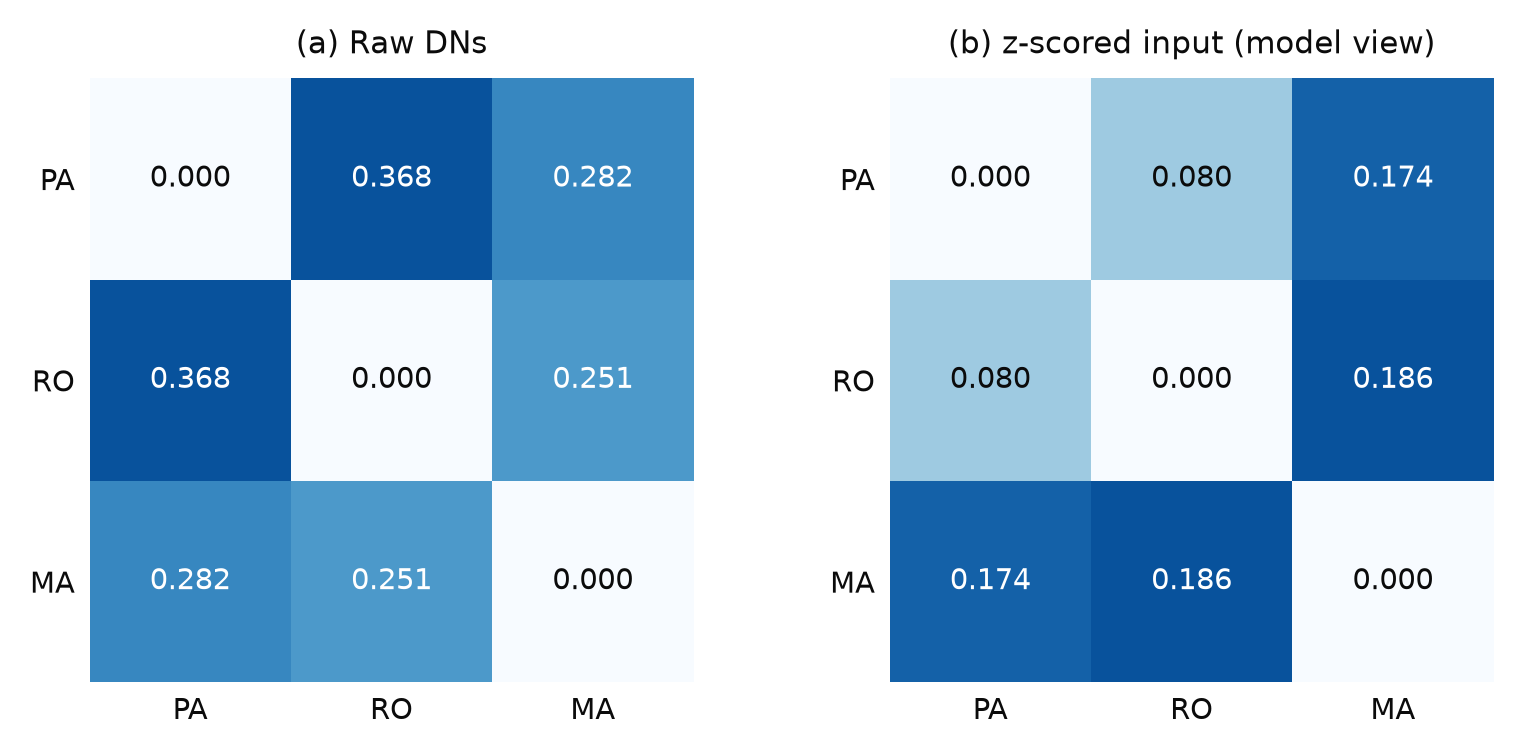
\includegraphics[width=0.75\textwidth]{figures/fig_spectral_distance.png}
\caption{Spectral distance between sites (mean absolute log-amplitude difference over 7 bands and 2 dates) on (a) raw DNs and (b) normalized inputs.}
\label{fig:distance}
\end{figure}

\subsection{Training dynamics}

Source validation loss reaches its minimum early.
The selected checkpoint is from epoch \BestEpMin{}--\BestEpMax{} (median \BestEpMed{}; epoch 1 for \BestEpOne{} of the \BestEpN{} distinct source-only models), and training stops at epoch \StopEpMin{}--\StopEpMax{}.
After that point, training loss keeps falling and validation loss rises.
Validation \Fone{} changes much less: its maximum over all epochs exceeds its value at the selected checkpoint by only \ValFGapMin{}--\ValFGapMax{}.
The model becomes more confident without becoming much more accurate on the source validation tiles.
The reported models are therefore early checkpoints.
A selection criterion based on validation \Fone{} or AP could pick different epochs, which we have not tested.

% ============================================================
\section{Discussion}\label{sec:discussion}

\textbf{What the simple methods buy.}
\BNTTA{} is nearly free and improves the ranking of target pixels in most pairs, but at a fixed threshold it can trade a large precision loss for a recall gain.
In practice it should be paired with a decision on the operating point, for example a threshold chosen to match a known deforestation rate, rather than applied with the source threshold.
FDA, once it actually swaps frequencies, is useful for one source domain (RO) and harmful for another (MA), so it is not a safe default either.
We can only speculate on why.
One possibility is that RO-trained source-only models are unstable across seeds on PA, and training on several styled versions of the scene acts as a regularizer that removes this instability.
Another is that MA's distinct low-frequency NIR content (Fig.~\ref{fig:spectra}) is overwritten by the swap.
Neither explanation is tested here.
Both cheap methods help on some pairs and hurt on others, and for both MA-source pairs no adaptation beats the unadapted model.
Choosing among them without target labels is itself an open problem; \citet{ortega2026domain} address a related question by estimating domain adaptation performance on the target from prediction uncertainty.

\textbf{Why reporting matters here.}
The seed spread we observe exceeds many of the method effects, and \Fone{} and AP can disagree on the sign of an effect.
A reliable comparison on this benchmark therefore needs several seeds, paired per-seed comparisons, and a threshold-free metric alongside \Fone{}.

\textbf{Limitations.}
(i) Three sites from one sensor and one year pair each; the results may not transfer to other regions, sensors or years.
(ii) Three seeds give a rough estimate of variance; we report counts rather than significance tests.
(iii) All metrics except AP use a fixed threshold of 0.5.
(iv) Checkpoints are selected by source validation loss and come from the first few epochs.
(v) \BNTTA{} statistics are estimated on the whole target scene, including test tiles (without labels).
(vi) The bottleneck uses a convolutional fallback instead of the intended Mamba block, so conclusions are about the network as run.
(vii) FDA is tested only at $\beta=0.01$, three styled versions and two mixing ratios.
(viii) Class weights are fixed at 0.4/2.0 rather than set from class frequencies.
(ix) Our tile assignment differs from the benchmark's fixed tiles, and our network (\ParamsM{}\,M parameters) is much smaller than the DeepLabv3+ variant of \citet{demoura2025enhancing} (more than 54\,M), so the absolute accuracy of our models is not comparable with theirs.

% ============================================================
\section{Reproducibility and Data Integrity}\label{sec:repro}

All runs use fixed seeds, and training is deterministic on our hardware (one NVIDIA RTX 4050 laptop GPU).
Every number in the text, tables and figures is generated by scripts from the logged per-run outputs.
While preparing this study we found that one working copy of the RO scenes and references had been damaged during a file copy.
The damaged files still loaded, but they held out-of-range values in place of image data, and models trained on them gave misleadingly poor RO results.
The data loader now rejects inputs whose image values fall outside the 16-bit range, whose no-data fraction exceeds 1\%, or whose reference rasters contain values other than 0 and 1.
All results reported here were produced after this check, with intact files.
We recommend similar checks to anyone reusing these data.

% ============================================================
\section{Conclusion}\label{sec:conclusion}

On three Landsat-8 deforestation sites, cross-domain \Fone{} without adaptation ranges from \SOMin{} to \SOMax{} and depends strongly on the direction of transfer.
Test-time BN adaptation improves average precision in most paired runs but changes \Fone{} at the default threshold by \TTAAllD{} on average, with losses on the pairs trained on MA.
FDA at the common $\beta=0.01$ does nothing on $64\times64$ patches; applied to scene tiles, it helps when training on RO, hurts when training on MA and does not improve AP overall, and fully styled training is not worse than a 50\% mix.
No configuration is best on all pairs, and on both MA-source pairs the unadapted model is best.
Because seed variance is comparable to the method effects, results on this benchmark should be reported over several seeds and with a threshold-free metric.


\backmatter

\bmhead{Acknowledgements}
This work builds on the author's Final Year Project at GIFT University, Gujranwala, Pakistan.

\section*{Statements and Declarations}

\bmhead{Funding} No funding was received for conducting this study.

\bmhead{Competing interests} The author has no relevant financial or non-financial interests to disclose.

\bmhead{Ethics approval and consent to participate} Not applicable.

\bmhead{Consent for publication} Not applicable.

\bmhead{Data availability} The Landsat-8 images and PRODES-derived reference maps of the three sites are the public benchmark data of \citet{noa2021adversarial} and \citet{demoura2025enhancing}, available from the links given by \citet{demoura2025enhancing}. The per-run results, logs and the tile split used here are available in the code repository below.

\bmhead{Code availability} The code for preprocessing, training, evaluation, the number-generation and audit scripts, and all figures is available at \url{https://github.com/ZentaCros/cross-biome-deforestation-da}.

\bmhead{Use of AI tools} The use of AI tools is described in Section~\ref{sec:impl}.

\bmhead{Author contribution} Muhammad Hamza Azeem: Conceptualization, Methodology, Software, Validation, Formal analysis, Investigation, Data curation, Writing -- review and editing, Visualization.

\bibliography{../references}

\end{document}
